\documentclass[11pt,dvipdfmx]{jreport}
\usepackage{amsmath,amssymb,amsfonts}
\usepackage{bm}
\usepackage{siunitx}
\usepackage[dvipdfmx]{graphicx}
\usepackage[top=30truemm,bottom=30truemm,left=25truemm,right=25truemm]{geometry}
\usepackage{comment}
\usepackage{jumoline} 
\usepackage{color}
% これより先に color と jumoline を読み込んでおく
%======================================
\newif\ifnoproofreadmark \noproofreadmarkfalse
\def\noproofreadmark{\noproofreadmarktrue}

\def\addspan#1{%
 \ifnoproofreadmark%
   #1%
 \else%
  \textcolor{red}{#1}%
 \fi%
}

\def\delspan#1{%
 \ifnoproofreadmark%
  \empty%
 \else%
  {\Midline{#1}}%
 \fi%
}

\def\delspanx#1{%
 \ifnoproofreadmark%
  \empty%
 \else%
  #1%
 \fi%
}

\def\strikemath#1{%
 \ifnoproofreadmark%
   \empty%
 \else%
   {\setjumocolor{red}\Midline{{\mbox{$\displaystyle #1$}}}}%
 \fi%
}
%=================================================
 %\noproofreadmark  % 最終原稿のときに有効化する

\MidlineHeight=0.5ex
\UMOlineThickness=0.2ex % お好みで決める


\title{
{\LARGE 修士論文\\[1cm]}
{\huge InGaAs系高利得量子井戸半導体レーザーの開発\\及び評価測定\\[1cm]
Development and characterization measurements of \\InGaAs high-gain quantum-well
lasers\\[5cm]}
}
\date{\LARGE 平成31年1月4日}
\author{\LARGE 東京大学大学院理学系研究科\\
\LARGE 物理学専攻\\[1cm]
\LARGE 指導教員 秋山 英文 教授\\[1cm]
\LARGE 学籍番号 35-176043\\
\LARGE 小松原 望}


\begin{document}
\maketitle			%タイトル
% !TEX root = main.tex
\begin{abstract}
  半導体レーザーは世の中で広く用いられている発光デバイスである。小型、高安定などの利点を有し非常に扱いが容易である。そのような半導体デバイスから直接ps程度の超短パルスを発生させることは、超短パルスを用いた様々な基礎研究の成果を技術的に応用する足がかりとなり得る。
 
% \addspan{本研究では応用上重要な電流注入型の1\si{ \micro\metre}波長帯InGaAs系半導体レーザーの高速化を目的として研究を行った。}
 %\addspan{1 \si{\micro\metre}波長帯InGaAs系半導体レーザーは、先行研究開発例が少ないため、設計・試作・評価計測を半導体の基礎物理に立ち戻って進める必要がある。}
 
 
 半導体から超短パルス光を得る手法として利得スイッチングを取り上げる。
 利得スイッチングはns程度の短い電気パルスを注入すること\addspan{で}それより短い数十ps\addspan{程度}の光パルスを得る技術である。電流による直接変調のみで実現可能であり\delspan{また}\addspan{、}複雑な構造を必要と\addspan{しない。したがって基本的な半導体内部のキャリアダイナミクスを直接反映する物理現象を理解することに繋がる。}\delspan{しないことから簡便に実現が可能な手法といえる。}
 %電流注入により半導体内部の利得を増幅し、反転分布を作る。
 
 利得スイッチング\delspan{パルスによる}\addspan{法を用いた}パルス発生に関しては古くから研究がなされてきているが、近年の研究\delspan{で}\addspan{において}光パルスの立ち上がりは半導体材料の\delspan{利得飽和}\addspan{飽和モード利得}が、立ち下がりは共振器寿命が決めているということが報告されている。共振器寿命は半導体レーザーの共振器長を短くすることで
 %\addspan{短くすることができ、
 \addspan{光パルスの}短パルス化が見込まれる。一方\addspan{飽和モード利得は}\delspan{利得飽和に関してはレーザーデバイス設計の時点では決めることができない。そこで利得飽和の代わりに}光閉じ込め係数を高くすることで高い利得を実現し\addspan{光}パルスの短パルス化を図れることが\addspan{GaAs系半導体レーザーの光励起実験などにより}示唆されている。
 
  \addspan{本研究では応用上重要な電流注入型の1\si{ \micro\metre}波長帯InGaAs系半導体レーザーの高速化を目的として研究を行った。}
 \addspan{利得スイッチング用1 \si{\micro\metre}波長帯InGaAs系半導体レーザーは、先行研究開発例が少ないため、設計・試作・評価計測を半導体の基礎物理に立ち戻って進める必要がある。}

\addspan{本研究では}量子井戸レーザーにおいて光閉じ込め係数は量子井戸の数を増やすことで実現される\addspan{ことに着目し、}\delspan{。}
\delspan{そこで本研究では10周期}多重量子井戸半導体レーザー\delspan{を}\addspan{の}デザインおよび開発を行った。\delspan{同時に3周期多重量子井戸レーザーも開発し}\delspan{、}%\addspan{た。}
\addspan{InGaAs系材料はGaAs基板に対する格子定数の違いからそのままでは量子井戸層の層数を大きくすることはできない。そこで格子定数の小さいInGaPをバリア層に用いることで10周期歪補償量子井戸レーザーを作製した。同時に歪補償を行わずに結晶成長させた3周期歪補償量子井戸レーザーの試作も行った。}

\addspan{作製したレーザーデバイスに対して}定常電流注入実験を行い\addspan{閾値電流及びスロープ効率の見積もりを行った。これらの値を解析することでモード利得が算出できる。10周期と3周期の2種類の井戸数のレーザーデバイスについて}比較したところ\addspan{、量子井戸の多重化によるモード利得の増大が確かめられた。}\delspan{高利得であることが示された。}
 
 また利得スイッチング動作を試みたところ10周期多重量子井戸レーザーでは最短で26.5 psというパルス幅を与えた。
 
 %共振器長あるいは量子井戸の層数を変えたことによる短パルス化の効果はあまり見られなかった。
\end{abstract}	%要旨
\tableofcontents 	%目次
\listoffigures 		%図目次
\listoftables 		%表目次

%%%%%%%%%%%%%%%%%%%%%%%%%%%%%%%%%%%%%%%%%%%%%%%%
%%%  本文
%%%%%%%%%%%%%%%%%%%%%%%%%%%%%%%%%%%%%%%%%%%%%%%

% !TEX root = main.tex
\chapter{序論}
\section{研究背景}
\subsection{半導体レーザー}
\subsubsection{半導体レーザーの現状}
半導体レーザーが実現されたのは1962年のことである 。キャリアと光の閉じ込めを能率よくできるようにした2重ヘテロ構造が用いられるようになり実用化・発展を遂げた。光通信、光ディスク用発光デバイスの核をなす技術である。他のレーザー\delspan{に}と比較しても小型・軽量、大量生産可能、熱や振動(安定性)に強いことなどが普及の主な理由である。近年では半導体からピコ秒程度の超短光パルスを発生させる技術も研究が盛んに行われており産業への応用が期待されている。
%[利得スイッチングsds生物発光yokoyamaさん,ここではGSにこだわらなくてもいいか][psパルスを使った産業]

\subsubsection{半導体レーザーの基礎特性}
%\addspan{半導体レーザーの定常発振条件について述べる。}
ここで半導体レーザーの特性について説明する。
まずは発振条件について述べる。
発振条件は共振器の中を往復する光が共振器を1周したときに元の光強度と同じであることである。これは式で表すと単位長さあたりの光損失$\alpha$ (/cm)、誘導放出による利得$g$ (/cm)、端面での反射率$R$(2つの端面の反射率を同じとした)を用いて
\begin{eqnarray}
\sqrt{R}\sqrt{R} \exp(-2\alpha L+ 2gL-i2\beta L)=1
\label{eq:1}
\end{eqnarray}
と書ける。$L$は共振器長\delsppp{である。}、$\beta$は伝搬定数、\adsppp{$i$は虚数単位}\delsppp{である。}\adsppp{を表す。}
この条件を満たす利得すなわち閾値利得は
\begin{equation}
g_{\rm{th}}=\alpha+\dfrac{1}{L}\ln\left(\dfrac{1}{R}\right)
\end{equation}
と書ける。また式(\ref{eq:1})の虚部が0になるという条件から
\begin{eqnarray}
2\beta L=2\pi m   (mは整数)
\end{eqnarray}
を得る。伝搬定数を2$\pi n_{\rm{eq}}/\lambda$と表すと、共振波長は
\begin{eqnarray}
\lambda =2n_{\rm{eq}}L/m
\end{eqnarray}
となる。$n_{\rm{eq}}$は
%光分布全体で空間積分した
等価屈折率である。

次にキャリアの再結合時間$\tau(n)$はバンド間の発光再結合寿命$\tau_{r}(n)$と非発光再結合寿命と$\tau_{nr} (n)$を用いて
\begin{eqnarray}
\dfrac{1}{\tau}=\dfrac{1}{\tau_{r}}+\dfrac{1}{\tau_{nr}}
\label{eq:tau_r}
\end{eqnarray}
で与えられる。$1/\tau_{n}$と$1/\tau_{nr}$はそれぞれ\addspan{発光再結合と非発光再結合の}割合であるから、内部量子効率$\eta_{int}$は全\delspan{キャリアの}再結合のうちの発光再結合の割合\delspan{であるから}\addspan{として}
\begin{eqnarray}
\eta_{int}=\dfrac{1/\tau_{r}}{1/\tau_{r}+1/\tau_{nr}}
\end{eqnarray}
で表される。
\subsubsection{超短パルス発生}
ピコ秒オーダーの超短パルスを発生する技術は長距離光ファーバー伝送\cite{ref_hasegawa}に加えて、精密レーザー加工\cite{ref_chichkov} や多光子励起顕微鏡を用いたバイオイメージングなど、応用の幅が広がってきている技術である。
%\addspan{領域}である。

半導体レーザーを用いた短パルス発生の代表的な方法としては利得スイッチングとモード同期法がある。利得スイッチング\cite{ref_h_ito}は注入電流を変調する直接変調の一種である。デバイスにナノ秒程度の電流パルスを注入すると励起パルスよりも短い、数十ピコ秒の光パルスが得られるというものである。半導体内の光強度が大きくなると誘導放出によってキャリアが消費され利得が急激に減少することにより光パルスが生じる。特徴としては複雑な構造を必要とせずほとんどの半導体レーザーで実現可能な技術であるという点である。

一方のモード同期法はサブps程度の超短パルスを得ることができる技術である。外部共振器あるいは共振器内に可飽和吸収体を挿入するなど付加的な構造が必要となる。

本研究では\delspan{比較的容易に実現できる}\addspan{半導体キャリアの高速ダイナミクス物理により直結した}利得スイッチングに注目する。
\begin{comment}
 半導体から短パルスを発生させる方法として従来行われてきた方法が主に3つある。モード同期法、Qスイッチ法、利得スイッチ法である。モード同期法は個体レーザーでも用いられておりフーリエ限界に近いパルス幅を生成できる反面パルスの繰り返し周期が固定されてしまうという特徴を持つ。一方Qスイッチング法は過飽和吸収帯を用いるなどしてQ値を瞬間的に増大させることで高エネルギーの光パルスを得ることができる。利得スイッチングは電流を変調する直接変調の一種であり、複雑な構造を必要とせず、全ての半導体レーザーで実現が可能な技術である。レーザー加工などの技術的応用においては繰り返し可変であることや様々な種類の光源を試すことができるという利点があるため、??本研究では利得スイッチング法に着目した。
\end{comment}


\subsubsection{利得スイッチング法}
利得スイッチングは1980年ごろに観測された\cite{ref_h_ito}\cite{ref_aspin}\cite{ref_torphammar}。光通信技術向上を念頭に置いた高周波変調技術の研究のなかで短パルス光が確認された。ItoらはAlGaAsレーザーに閾値以下のDCバイアスと100$\sim$300MHzの高周波変調を重層することで時間幅約30 ps光パルスが発生できることを報告した。その後電源として用いるパルスジェネレーターの進歩などにより研究が進み報告も盛んに行われてきた。
約5 psの非常に短い報告もなされている\addspan{\cite{ref_nagarajan}}。\adsp02{Chenらは1.55 \si{\micro\metre}波長帯において電流注入利得スイッチングパルスの高周波成分を切り出すことで4.7 psのパルス幅の実現を報告している\cite{chen_yokoyama}。}
%図\ref{fig:fig_1_1_GS_ito}bに過去40年間に報告されてきた利得スイッチングのパルス幅がプロットされている。赤が光励起、青が電流注入を表している。電流注入の報告を見てみると最短でも5ps程度である。

また応用としては利得スイッチングを利用した生物発光イメージの撮像の報告がある\cite{ref_h_yokoyama}。


次に利得スイッチングの基本的な動作について述べる。


利得スイッチング\adsp02{の基本}動作は半導体中のレーザー動作特性を記述する\adsp02{シングルモード}レート方程式により理解されている\cite{ref_lau}。
レート方程式はデバイス中のキャリア密度と光子密度の時間変化の振る舞いを以下のような連立方程式で表している。$ n$ は量子井戸1層あたりのキャリア密度、$s$ は光子密度を表す。式(\ref{eq:late_eq_1})はキャリア密度 の時間変化を記述している。右辺第1項は外部から注入されるポンプキャリア、第2項は誘導放出、第3項は自然放出を表す。式(\ref{eq:late_eq_2})は光子密度の時間変化を記述しており、第1項は誘導放出による増幅、第2項は共振器寿命による減衰、第3項は自然放出光を表す。
\begin{eqnarray}
\label{eq:late_eq_1}
\dfrac{dn}{dt}&=&n_{\rm{pump}}\zeta(t)-\dfrac{\Gamma}{m}\nu_{\rm{g}}g(n)\dfrac{s}{1+\epsilon s}-\dfrac{n}{\tau_{r}}\\
\dfrac{ds}{dt}&=&\Gamma\nu_{g}g(n)\dfrac{s}{1+\epsilon s}-\dfrac{s}{\tau_{p}}+m\beta\dfrac{n}{\tau_{r}}
\label{eq:late_eq_2}
\end{eqnarray}
\begin{eqnarray*}
&n& : 量子井戸1層あたりのキャリア密度 [\rm{m^{-3}}]\\
&s& : 活性層全体の光子密度[\rm{m^{-3}}]\\
&n_{\rm{pump}}& : 励起キャリア密度 \\
&\zeta(t)& : 規格化された励起パルスの時間変化\\
&\Gamma & : 光閉じ込め係数\\
&m& : 量子井戸数\\
&\nu_{g}& : 群速度[\rm{m/s}]=c/n_{eq}\\
&g(n)& : 利得[\rm{cm^{-1}}]\\
&\epsilon & : 利得圧縮係数\\
&\tau_{r}& : キャリアの発光再結合寿命[\rm{s^{-1}}]\\
&\tau_{p}& : 共振器寿命 [\rm{s^{-1}}]\\
&\beta& : 自然放出光係数\\
\end{eqnarray*}
共振器寿命$\tau_{p}$は
%ファブリー・ペローレーザーの場合
\begin{eqnarray}
\tau_{p}=\dfrac{n_{\rm{eq}}}{c(\alpha+\rm{ln}  (1/\it R)/L)}
\label{eq:tau_p}
\end{eqnarray}
とかける\cite{ref_iga}。
$n_{\rm{eq}}$は等価屈折率、$\alpha$は共振器内部の光損失、$c$は光速、$L$は共振器長、$R$は共振器のミラー端面の反射率である。
\begin{comment}
\subsubsection{半導体レーザーの特性}
半導体レーザーの基本的な特性について説明する。
まずは発振条件について述べる。
発振条件は共振器の中を往復する光が共振器を1周したときに元の光強度と同じであることである。\delspan{これは}式で表すと単位長さあたりの光損失$\alpha$ (/cm)、誘導放出による利得$g$ (/cm)、端面での反射率$R$(2つの端面の反射率を同じとした)を用いて
\begin{eqnarray}
\sqrt{R}\sqrt{R} \rm{exp}(-2\alpha L+ 2gL-i2\beta L)=1
\label{eq:1}
\end{eqnarray}
と書ける。$L$は共振器長である。$\beta$は伝搬定数である。
この条件を満たす利得すなわち閾値利得は
\begin{equation}
g_{\rm{th}}=\alpha+\dfrac{1}{L}\rm{ln}\left(\dfrac{1}{R}\right)
\end{equation}
と書ける。また式(\ref{eq:1})の虚部が0になるという条件から
\begin{eqnarray}
2\beta L=2\pi m   (mは整数)
\end{eqnarray}
を得る。伝搬定数を2$\pi n_{\rm{eq}}/\lambda$と表すと、共振波長は
\begin{eqnarray}
\lambda =2n_{\rm{eq}}L/m
\end{eqnarray}
となる。$n_{\rm{eq}}$は光分布全体で空間積分した透過屈折率である。

次にキャリアの再結合時間$\tau(n)$はバンド間の発光再結合寿命$\tau_{r(n)}$と非発光再結合寿命と$\tau_{nr}(n)$を用いて
\begin{eqnarray}
\dfrac{1}{\tau}=\dfrac{1}{\tau_{r}}+\dfrac{1}{\tau_{nr}}
\label{eq:tau_r}
\end{eqnarray}
で与えられる。$1/\tau_{n}$と$1/\tau_{nr}$はそれぞれ割合であるから、内部量子効率$\eta_{int}$は全キャリアの再結合のうちの発光再結合の割合であるから
\begin{eqnarray}
\eta_{int}=\dfrac{1/\tau_{r}}{1/\tau_{r}+1/\tau_{nr}}
\end{eqnarray}
で表される。
\end{comment}
%\subsubsection{利得スイッチング}
上式のようなレート方程式を基に短い励起パルスを印可した時の発光および利得の時間変化についてシミュレーションを行った結果を図\ref{fig:fig_1_1_GS_ito}aに示す。赤線が光励起によるインパルス励起の様子、青線が電流注入による数 ナノ秒パルス励起の様子である。青線に注目すると図\ref{fig:fig_1_1_GS_ito}a上段での励起パルスよりも短い、数十 ピコ秒光パルスが出てくることがわかる。さらに1つ目のパルスの後は緩和振動が起きている。これが典型的な利得スイッチング動作である。また下段には利得の時間変化が示されている。励起が始まると同時に電子密度つまり利得が増えていき、ある時刻をすぎると閾値に達し反転分布を形成する。今度は誘導放出によって一気にキャリアが消費される。このキャリアの消費が注入されるキャリアよりも大きくなるため、利得も急激に減衰し光パルスも\delsppp{光子}\adsppp{共振器}寿命程度で立ち下がる。これが利得スイッチングの大まかな理解である。

\begin{figure}[h]
	\centering
	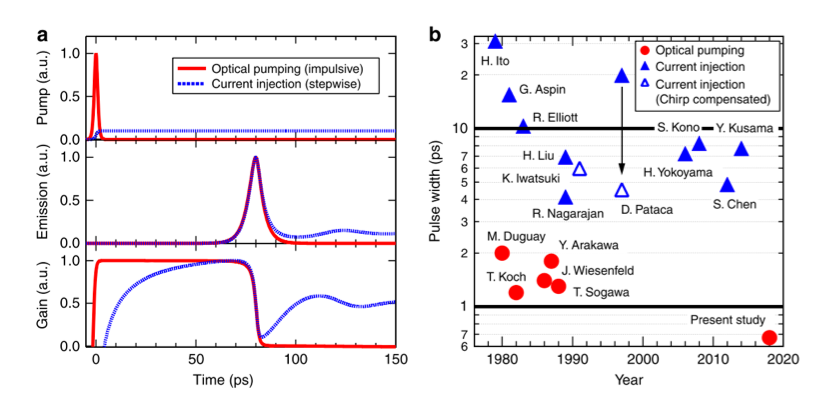
\includegraphics[width=15cm]{figure/fig_1_1_GS_ito.png}
	%\centering
	\caption[典型的な利得スイッチングパルスの時間変化と先行研究におけるパルス幅]	{典型的な利得スイッチングパルスの時間変化と先行研究におけるパルス幅の報告
	\protect\newline a 利得スイッチングパルスの時間変化、b先行研究におけるパルス幅\cite{ref_t_ito}}
	\centering
	\label{fig:fig_1_1_GS_ito}
\end{figure}

\newpage
\subsubsection{利得スイッチングパルスの詳細な理解}
%利得スイッチング光パルスのより詳細な理解を視覚的に表したのが図\ref{fig:fig_1_1_GS_pulse}である\cite{ref_1_1_GS}である。
\begin{figure}[ht]
	\centering
	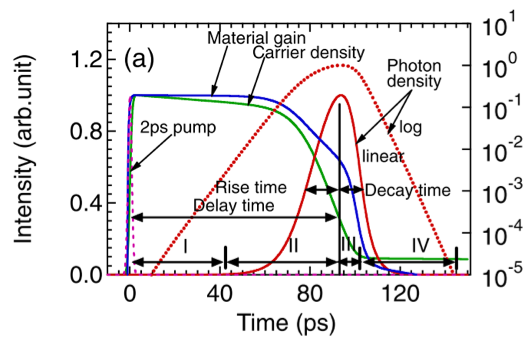
\includegraphics[width=15cm]{figure/fig_1_1_GS_pulse.png}
	\caption[パルス生成中のキャリア密度、光子密度、材料利得の時間変]{パルス生成中のキャリア密度、光子密度、材料利得の時間変化\cite{ref_1_1_GS}}
	\label{fig:fig_1_1_GS_pulse}
\end{figure}

レート方程式の誘導放出の項に関わってくる材料利得$g(n)$はキャリア密度$n$に比例する線形利得$g_{0}(n-n_{0})$の形で近似されてきた($g_{0}$は利得定数、$n_{0}$は透明キャリア密度)。しかし高密度励起領域では線形利得では説明できないことがわかり、非線形な効果を取り入れた利得の形が提唱された。その1例を示す。Chenらは$g(n)$に式(\ref{eq:nonlier_gain})のように非線形な項を取り入れ、数値計算を行った\cite{ref_1_1_GS}。線形な項に加えて$g_{s}$といった利得飽和の効果を取り入れている。図\ref{fig:fig_1_1_GS_pulse}にこの時のパルス生成中のキャリア密度、光子密度および利得の時間変化を示す。時刻0で2 psのインパルス励起行った時の光の時間波形赤の実線と破線、キャリア密度を緑の線、材料利得を青い線で表している。
\begin{eqnarray}
\label{eq:nonlier_gain}
g(n)&=&g_{0}(n-n_{0})\left[1+\dfrac{g_{0}(n-n_{0})}{g_{s}}\right]^{-1}\\
&\simeq &\left\{
\begin{array}{ll}
 g_{0}(n-n_{0}) & n-n_{0}\ll g_{s}/g_{0}\nonumber \\
g_{s} & n-n_{0}\gg g_{s}/g_{0}\nonumber
\end{array}
\right.
\end{eqnarray}
図\ref{fig:fig_1_1_GS_pulse}においてIとIIの領域つまり立ち上がりの時間領域では光子密度が小さい一方でキャリア密度が大きいため、$g_{s}$が支配的に立ち上がりのはやさの限界を決めている。IIIの領域ではキャリア密度が小さく、光強度が大きい領域であり$\epsilon$が効いてくる。IVの領域ではキャリア密度も光子密度も小さくなっているため減衰のはやさは光子の共振器寿命$\tau_{p}$によってきまる。

つまり利得スイッチングパルスのパルス幅は立ち上がりのはやさの限界を\delspan{利得飽和}\addspan{飽和モード利得}$\Gamma g_{s}$、立ち下がりのはやさの限界を共振器寿命$\tau_{p}$が決めている。
\newpage

\subsubsection{利得スイッチングパルスの短パルス化}
利得スイッチングパルスの短パルス化のためには\delspan{利得飽和}\addspan{飽和モード利得}$\Gamma g_{s}$を大きくすることと共振器寿命$\tau_{p}$を短くすることが必要であると示唆された。
\begin{comment}


共振器寿命$\tau_{p}$はファブリー・ペローレーザーの場合
\begin{eqnarray}
\tau_{p}=\dfrac{n_{\rm{eq}}}{c(\alpha_{a}+\rm{ln}(1/R)/L)}
\label{eq:tau_p}
\end{eqnarray}
とかける\cite{ref_iga}。
$n_{\rm{eq}}$は等価屈折率、$\alpha_{a}$は共振器内部の損失、cは光速、Lは共振器長、Rは共振器のミラー端面の反射率である。
\end{comment}
\addspan{式}(\ref{eq:tau_p})を見ると$\tau_{p}$を小さくするためには端面反射率$R$を小さくすること\addspan{あるいは}共振器長$L$を短くなるようレーザー設計することが有効であるとわかる。
通常端面反射率を下げるためには誘電体膜をコーティングする手法が用いられる。コーティングは光の高出力化のためにも用いられている一般的な手法である。


\delspan{この段落大きく変えた}


\begin{comment}
\delspan{利得飽和}\addspan{飽和利得}$g_{s}$は\addspan{単層の活性層}\delspan{用いる}材料によって決定されるパラメータである\delspan{ためデザインの段階で決めることはできない。そこで式(\ref{eq:late_eq_2})の第1項、誘導放出の項に注目してみると$g(n)$の代わりに}\addspan{一方で$\Gamma$は全体の構造によって決まる。}を大きくすることが有効であるとわかる。\addspan{モード利得}$\Gamma g(n)$を大きくすることができるためである。$\Gamma$が大きくなるような\delspan{結晶}\addspan{全体}構造をデザインすることが利得スイッチングパルスの短パルス化につながる。\addspan{本研究では伊藤らが行った\cite{ref_t_ito}ような飽和利得$g_{s}$の領域については考えず、光閉じ込め係数$\Gamma$を増大させることによるモード利得$\Gamma g$の増大について考える。}
%多重量子井戸にすることと$g_{s}$には関係があるんだっけ?ない
%このように利得スイッチングには興味深い非線形性が含まれており詳細に理解を進めることは半導体レーザーそのものの理解にも繋がりうる。
\addspan{飽和利得}$g_{s}$は単層の活性層材料によって決定されるパラメータである。一方光閉じ込め係数$\Gamma$はウエハ全体の構造によって決定される。
\end{comment}
\addspan{飽和利得$g_{s}$は量子井戸の活性層材料によって決定されるパラメータである。一方光閉じ込め係数$\Gamma$はデバイス構造によって決定される。構造を工夫することで光閉じ込め係数$\Gamma$を大きくすることが可能である。本研究では伊藤ら\cite{ref_t_ito}が光励起実験で示した飽和利得$g_{s}$の影響が現れるような領域については考えず、光閉じ込め係数$\Gamma$を増大させることによるモード利得$\Gamma g$の増大について考える。}
\clearpage
\subsection{InGaAs高利得材料}
先の節で\addspan{モード利得を大きく}\delspan{高利得化}することによ\delspan{る}\addspan{り}利得スイッチングパルスの高速化が見込めることについて述べた。またデバイスの構造を工夫することで光閉じ込め係数を増大させ、モード利得$\Gamma g$を高くすることを目指すと述べた。

本項ではデバイスの構造について具体的に述べる。量子井戸レーザーにおいては多重量子井戸化を
%\delspan{持ちた}\addspan{用いた}
行うことによる光閉じ込め係数の増大について述べる。合わせて多重量子化の結晶成長の\delspan{の}際に生じる結晶の歪みについても述べる。
\subsubsection{量子井戸レーザー}
まず量子井戸レーザーであるが
%井戸の中の電子のエネルギーが離散値をとるので発振波長の短波長化が図れる(どうでもよくない?)
、閾値電流密度の温度変化が小さい(バンド端の状態密度が大きいことに由来)、再結合効率が大きい(キャリアが量子井戸に閉じ込められることに由来)などの特徴を有する。


量子井戸レーザーは1975年Van der ZielらによってMBEにより作られた\cite{ref_van}。DupuisらはMOCVD法により量子井戸レーザーの作製を行い閾値電流の温度依存性が量子井戸レーザーでは抑えられることなどを指摘した\cite{ref_dupuis}。%T_{0}がでかい
MBEやMOCVDの発展により様々な材料の量子井戸レーザーが作られている。
%閾値電流密度が実現され注目を集めたのち、
%その後Tsangにより$0.25kA/cm^{2}$の程閾値電流密度をもつ量子井戸レーザーが発表され注目を集めた。近年では様々な材料の量子井戸レーザーが作られている。
\subsubsection{多重量子井戸レーザー}
量子井戸レーザーの特徴の1つとして量子井戸の厚さ、量子井戸の数のデザインが可能である、という点があげられる。ここで量子井戸の数mに注目する。単一量子井戸とm周期多重量子井戸を比較した場合、透明電流はm倍になる反面、第一サブバンドに収容できるキャリアの数がm倍になるためモード利得(光閉じ込め係数$\Gamma$×材料利得$g$)もm倍になることが予想される。
%しかしこれは材料利得が線形であることを想定した場合であり、利得の平坦化を考えると図のようにgが変化することが計算されている。[]目指す利得によって適切な井戸数を選ぶ必要があることを示唆している。

m周期多重量子井戸レーザーと単一量子井戸レーザーを比較した場合を考える。
半導体レーザーの発振条件は誘導放出の\addspan{モード}利得\delspan{(光閉じ込め係数 × 材料利得)}が全体の損失$\alpha^{total}$に等しいというものであるから、
%\begin{eqnarray}
%\Gamma g_{mod}=\alpha^{total}= \xi a_{\rm{ac}} +(1-\xi)a_{\rm{ex}}+\rm{ln}(1/R)/L
%\end{eqnarray}
\begin{eqnarray}
\label{eq:th}
\Gamma g_{\rm{material}}&=&\alpha^{\rm{total}}= \Gamma \alpha_{\rm{ac}} +(1-\Gamma)\alpha_{\rm{ex}}+\dfrac{1}{L}\rm{ln}\left( \dfrac{1}{\it R} \right )\\
&=& \alpha + \dfrac{1}{L}\rm{ln}\left( \dfrac{1}{\it R} \right )
%\Gamma g_{\rm{material}}=\alpha^{\rm{total}}= \alpha +\dfrac{1}{L}\rm{ln}\left( \dfrac{1}{R} \right )
\end{eqnarray}

と書ける。
$\alpha_{\rm{ac}}$はキャリアが注入される活性層(active layer)の損失、$\alpha_{\rm{ex}}$はクラッド層およびバリア層の損失の平均を表す。その2つを合わせて導波路内部の光の損失を$\alpha$とする。
$L_{z}$を量子井戸の厚さ、光導波路モードの実効的な広がりの厚さを$L_{0}$とすると、$L_{z}\ll L_{0}$の場合光閉じ込め係数$\Gamma$は近似的に
\begin{equation}
\Gamma = mL_{z}/L_{0}
\label{eq:Gamma}
\end{equation}
と書ける。$L_{0}$は典型的に0.1$\ \si{\micro\metre}$程度である。
一方注入電流密度にについては多重量子井戸でも単一量子井戸でも活性層一層あたりでは等しいとして
\begin{equation}
J_{m}=mJ_{m=1}
\label{eq:J_M}
\end{equation}
という関係がある。注入電流密度はキャリア面密度Nを用いて
\begin{equation}
J_{m=1}=eN/\tau_{r}
\end{equation}
と表せる。式(\ref{eq:J_M})はm周期多重量子井戸はm倍のモード利得が得られることを意味する。その反面発振に必要な注入電流もm倍になる。単一量子井戸の材料利得が注入電流と線形な関係にあると仮定すると
\begin{eqnarray}
g_{\rm{material}}=a(J_{m=1}-J_{g})
\label{eq:g_lineier_g}
\end{eqnarray}
と書ける($J_{g}$は利得が0となる透明条件を与える透明電流密度、aは係数)。単一量子井戸レーザーの閾値電流密度$J^{\rm{th}}_{m=1}$は式(\ref{eq:th})の左辺$g_{\rm{material}}$に式(\ref{eq:g_lineier_g})を代入し$\Gamma$に式(\ref{eq:Gamma})を代入して変形すると
\begin{eqnarray}
J^{\rm{th}}_{m=1}&=&\alpha^{total}/ a\Gamma + J_{g}\nonumber\\
&=&\alpha^{total}/(aL_{z}/L_{0})+J_{g} 
\end{eqnarray}
と書ける。また多重量子井戸レーザーでは式(\ref{eq:J_M})より
\begin{equation}
J_{m}^{t\rm{h}}=\alpha^{totla}/(aL_{z}/L_{0}) + mJ_{g}
\label{eq:Mj0}
\end{equation}
となる。常に単一量子井戸レーザーの方が低い閾値電流密度を与えることになる。これは材料利得が注入電流に対して線形な場合の結論である。
実際には励起強度を上げていくと
%(つまり擬似フェルミ準位を増加させていくと)サブバンド端では
利得が飽和することが知られている。
図\ref{fig:fig_gain_mode}に量子井戸層の数を変えたときのモード利得と注入電流の関係を示す\cite{y_arakawa}。横軸が注入電流密度、縦軸がモード利得である。電流密度が小さいときには井戸数が少ない方がモード利得が大きい。しかし電流密度を大きくしていくと井戸数が多い方が高いモード利得を得られることが数値計算によって示された。
 %モード利得が共振器の正味の損失$\alpha^{\rm{total}}$に等しくなると発振を開始する。そのため、$\alpha^{\rm{total}}$が大きいようなデバイスにおいては多重量子井戸構造の方が高いモード利得を得られるため閾値電流を下げるのには有利である。また電流量を増やしていくと
\begin{figure}[h]
	\centering
	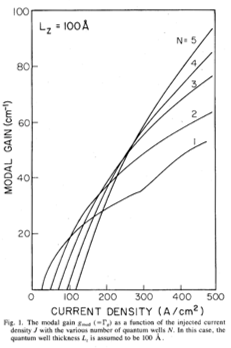
\includegraphics[width=5cm]{figure/fig_1_1_gain_mode.png}
	\caption{量子井戸層の数を変えたときのモード利得と注入電流の関係}
	\label{fig:fig_gain_mode}
\end{figure}


%モード利得のずほしい


%言いたいこと
%要は多重にするとモード利得が大きくなるため高速化に適している。

\subsubsection{量子井戸レーザーにおける歪効果}
前節で多重量子井戸化することで高利得化を実現できることを述べた。
しかし活性層とバリア層の結晶格子定数が異なる場合歪が発生する。このため活性層を厚く積むと歪が蓄積され結晶に欠陥・転移ができてしまう。


本節では多重歪量子井戸レーザーを紹介し、また多重量子井戸化における歪の影響について述べる。
歪量子井戸は活性層とバリア層あるいはクラッド層の結晶格子定数に違い(格子不整合)により歪が発生することを利用した量子井戸構造である。層の厚さが数nmの薄膜になると内部に歪を含んだままミスフィット転移を起こさずに膜を成長させることができ歪量子井戸を作ることができる。
\begin{figure}[h]
	\centering
	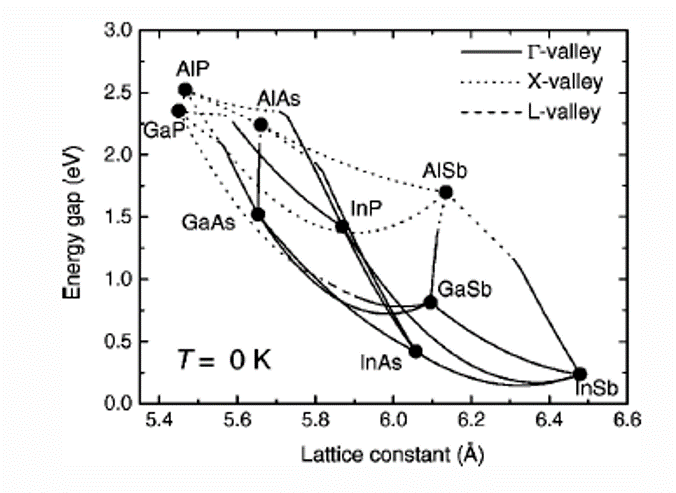
\includegraphics[width=13cm]{figure/fig_1_1_lattice_constance.png}
	\caption[III-V族原子の格子状数とバンドギャップの関係]{III-V族原子の格子状数とバンドギャップの関係\cite{ref_band_para}}
	\label{fig:fig_1_1_lattice_constance}
\end{figure}

一般にヘテロ\delspan{結合}\addspan{構造材料}においては格子定数が異なる。
図\ref{fig:fig_1_1_lattice_constance}にIII-V族原子の格子状数とバンドギャップの関係を示す\cite{ref_band_para}。例えばGaAsの格子定数は5.65 \AA 、 InAsの格子定数は6.06 \AA と0.4 \AA 程度大きいことがわかる。GaAsに対してInAsは約7\%格子定数が大きい。またInGaAsもGaAsよりも格子定数が大きい。InGaAsをGaAsに格子整合させながら結晶成長させようとした場合、格子定数の大きいInGaAsがどのように歪むかを図\ref{fig:fig_lattice_strain02}に模式的に示す。井戸方向には圧縮され、積層方向には引っ張られるように変形する。
ヘテロ界面に平行な井戸方向の面内歪を$\epsilon_{\|}$、垂直な歪を$\epsilon_{\bot}$とした。

基板の格子定数をa、 活性層の格子定数を$a+\Delta a$とすると
歪は
\begin{eqnarray}
\epsilon_{\|}&=&\epsilon_{xx}=\epsilon_{yy}=-\dfrac{\Delta a}{a}\\
\epsilon_{\bot}&=&\epsilon_{zz}=-\dfrac{2C_{12}}{C_{11}}\epsilon_{\|}\simeq -\epsilon_{\|}
\end{eqnarray}
と書ける。$\epsilon_{\|}<0$が圧縮歪、$\epsilon_{\|}>0$が引っ張り歪に対応する。$C_{11}$と$C_{12}$は弾性定数と呼ばれる値で通常正四面体結晶構造の半導体では$C_{11}\simeq 2C_{12}$の関係が成り立つ\cite{ref_iga}。


このとき体積変形(静水圧変形)と軸方向変形の合成を見ると
\begin{eqnarray}
\epsilon_{\rm{vol}}&=&\Delta V/V=\epsilon _{xx}+\epsilon _{yy}+\epsilon_{zz}\simeq \epsilon_{\|}\\
\epsilon_{\rm{ax}}&=&\epsilon_{\bot}-\epsilon_{\|}=-\dfrac{C_{11}+2C_{12}}{C_{11}}\epsilon_{\|}\simeq 2\epsilon_{\|}
\end{eqnarray}
と書ける。
\begin{figure}[h]
	\centering
	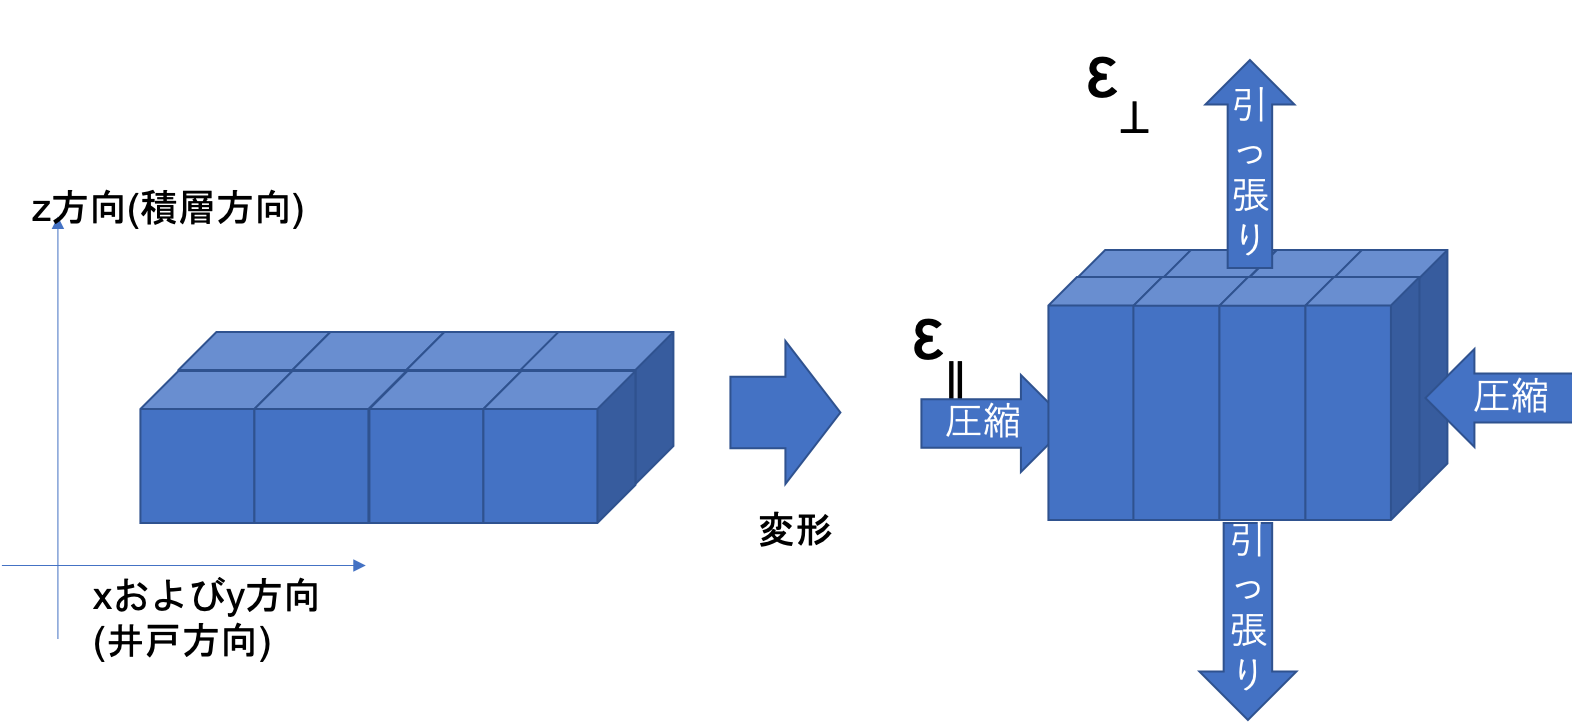
\includegraphics[width=10cm]{figure/fig_1_1_lattice_strain02.png}
	\caption{歪の模式図}
	\label{fig:fig_lattice_strain02}
\end{figure}
歪の発生により結晶内部に応力エネルギーが蓄えられる。このエネルギーが転移の発生に必要なエネルギーを超えなければ結晶は安定となる。応力エネルギーは膜厚に比例するため転位が発生しない最大の膜厚が存在する。これを臨界膜厚と呼ぶ。

図\ref{fig:fig_1_2_strain_vs_d}にInGaAs/GaAs歪超格子のInGaAs層における歪と膜厚、結晶性の関係を示す\cite{ref_konagai}。実線は理論的に導かれた臨界膜厚である。プロットはフォトルミネッセンスおよびホール測定などにより結晶性を調べたもので、黒プロットは高品質と判断されるもの、白抜きプロットは結晶性が劣ると判断されるものである。これらを見ると実験と理論がよく一致しており臨界膜厚以上の厚さでは結晶性が低下することがわかる。

\begin{figure}[h]
	\centering
	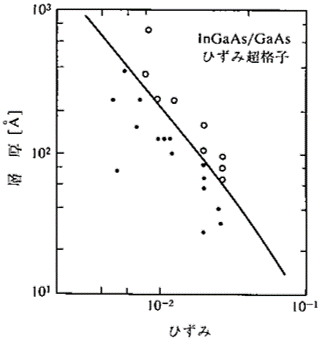
\includegraphics[width=9cm]{figure/fig_1_2_strain_vs_d.png}
	\caption[InGaAs/GaAs歪超格子のInGaAs層における歪と膜厚、結晶性の関係]{InGaAs/GaAs歪超格子のInGaAs層における歪と膜厚、結晶性の関係
	\protect\newline 実線 : 臨界膜厚の理論曲線、白抜きプロット : 結晶性が劣る、黒プロット : 高品質}
	\label{fig:fig_1_2_strain_vs_d}
\end{figure}
\begin{comment}
Matthewsらは多重薄膜構造において転移の発生しない限界の層厚$H_{c}$を理論的に次のように導いている。\cite{ref_Matthews}
\begin{eqnarray}
h_{c}=\dfrac{b(1-\nu \cos ^2 \alpha)}{2\pi f (1+\nu ) \cos \lambda}\left(\rm{ln}\dfrac{h_{c}}{b}+1\right)
\end{eqnarray}

ここで$b=a\sqrt{2}$、$f=2\epsilon$、$\nu$ : ポアソン比、$\alpha$ : 転移線とバーガースベクトスのなす角、$\lambda$ : すべり面と海面の光線に垂直な面の方向をすべり面の方向のなす角である。
\end{comment}

次に歪がある場合のバンド構造の変化および歪量子井戸レーザーの特性について定性的に述べる。

体積変形歪みは伝導帯と価電子帯のバンド端をシフトさせバンドギャップ$E_{g}$を$\Delta E_{g}=a\epsilon_{\rm{vol}}$だけ変化せさせる。aは静水圧変形ポテンシャル(hydrostatic deformation potential)と呼ばれる定数である。GaAsでは2.7 eV、InAsでは2.5 eV報告されている\cite{ref_adachi}。一方軸性変形歪は価電子帯の構造を変化させ、量子井戸レーザーの特性変化の主要因となっている。歪がない半導体では価電子帯の頂上はヘビーホールとライトホールが縮退しているが、軸性歪により縮退が解けてそれぞれの頂上が上下反対方向にシフトする。バンドの分離量は$E_{ll-hl}\simeq -2b\epsilon_{\rm{ax}}$で与えられる。bは軸性変形ポテンシャルと呼ばれる。


%ここに$k_{\|}$方向の図ほしい

圧縮歪の場合、一番上の量子化準位の$k_{\|}$方向のバンド構造はライトホールになっている。すると有効質量が小さく、すなわち状態密度が小さい。するとキャリア注入による擬フェルミ準位の変化が大きくなり反転分布が生じやすくなる。(反転分布の条件:$E_{fc}-E_{fv}>h\omega _{p}\geq E_{g}$を達しやすくなる)したがって発振閾値が無歪に比べて小さくなる。引っ張り歪の場合準位間分離が大きくなると価電子帯混合の影響が減って$k_{\|}$方向の有効質量が小さくなる。これにより閾値を下げることが可能である。光ファイバ通信用の1.55\ $\si{\micro\metre}$帯で低い閾値電流密度が報告されている\cite{ref_thijs}。図\ref{fig:fig_lattice_strain_Ith}に歪の異なるレーザーについての閾値電流密度を共振器長の逆数に対してプロットした図を示す。この報告の中ではInP基板の上に$\rm{In_{x}Ga_{1-x}As}$を結晶成長させたレーザーを用いている。引っ張り歪みが0, 1.1, 1.5, 2.2の単一量子井戸レーザーについて歪が大きいほど閾値電流が低くなることを報告した。図\ref{fig:fig_lattice_strain_Ith}において歪が0, 1.1, 1.5と大きくなるにしたがって閾値電流密度は小さくなっている。歪が2.2の場合にはミスフィット転移が生じたため閾値電流密度が高くなってしまった。

このように歪を利用することで半導体のバンド構造を変化させ高性能なレーザーを開発する研究が行われてきた。
\begin{figure}[h]
	\centering
	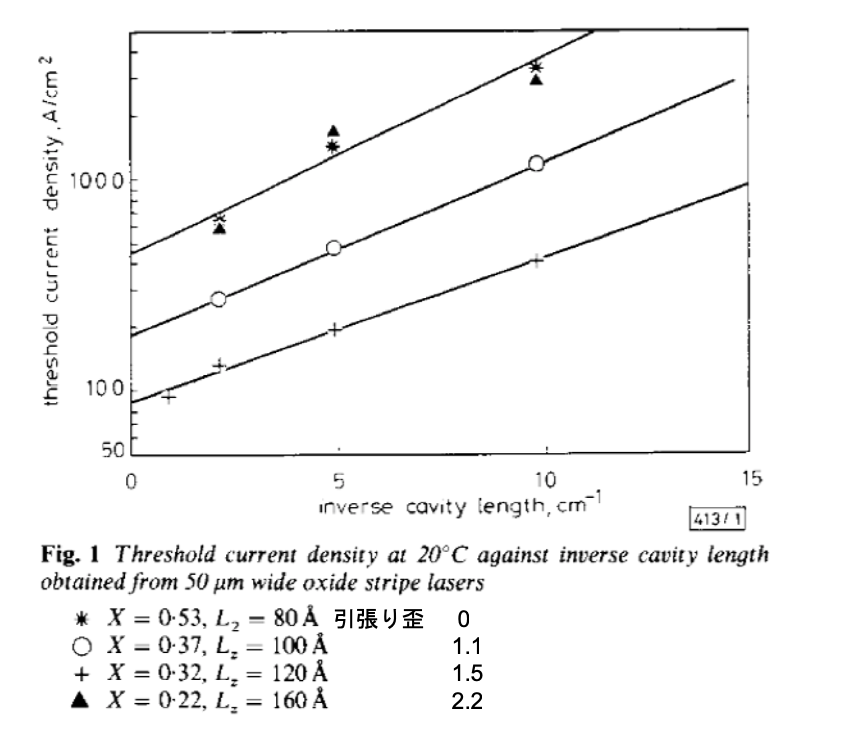
\includegraphics[width=10cm]{figure/fig_1_1_lattice_strain_Ith.png}
	\caption[単一歪み量子井戸レーザーの閾値電流密度]{単一歪み量子井戸レーザーの閾値電流密度\cite{ref_thijs}}
	\label{fig:fig_lattice_strain_Ith}
\end{figure}

%じゃあ3QWの利得計算してみれば?ってなるよね
\clearpage
\subsubsection{InGaAs歪補償レーザー}
%式(\ref{eq:Gamma})からわかるように多重量子化することで光閉じ込め係数を増大させ正味の利得を増やすことができる。
多重量子井戸化を行うにも格子不整合による歪が生じるために量子井戸層を積むことのできる限界の厚さが存在することを前節で述べた。


井戸層の歪をバリア層で補償する歪補償量子井戸が導入された。図\ref{fig:fig_1_1_lattice_constance}の格子定数とバンドギャップの関係の図を見ると、InGaAsはGaAsよりも格子定数が大きく、GaAsPは小さいことがわかる。GaAsに格子整合する際に\rm{InGaAs}層とGaAsP層をnmスケールで交互に結晶成長することで\rm{InGaAs}に生じる圧縮歪をGaAsPに生じる引張り歪で相殺しながら結晶成長することができる。
歪補償の条件は以下の式で表される。井戸層の格子定数および厚みを$a_{well}$、$L_{well}$、バリア層の格子定数と厚みを$a_{barrier}$、$L_{barrier}$とする。
\begin{eqnarray}
<a>=\dfrac{a_{well}L_{well}+a_{barrier}L_{barrier}}{L_{well}+L_{barrier}}=a_{substrate}
\label{eq:conpensate}
\end{eqnarray}
歪補償を行った格子整合の模式図を図\ref{fig:fig_1_1_lattice_strain_comp}に示す。このように格子整合を行うことで量子井戸数を増加させることができる。


歪補償により微分利得の増加の報告もある\cite{ref_Dutta}。DuttaらはInGaAs/GaAs系3周期歪量子井戸レーザーとInGaAs/GaAsP系4周期歪補償量子井戸レーザーの線形利得をそれぞれ$dg/dn$=1.0$\times 10^{-15}\rm{ cm^{2}}$と$dg/dn$=2.1$\times 10^{-15}\rm{ cm^{2}}$と見積もっている。

%歴史的には歪補償を行うことにより発光スペクトルおよび吸収スペクトルの長波長化も目的とされていた。
%歪み補償は\cite{ref_t_kawamura}
%歪み補償の説明→歪み補償を使ったレーザー→高利得のレーザー作った人いるかな
%どういう目的今まで歪補償レーザーが作られてきたのか?
%(温度特性300K以上の閾値電流の温度依存性の小さいレーザーが実現された[T.Hayakawa])余裕があったら入れる
%g_{0}が大きくなることを言cちゃダメかも
%Yb ドープファイバーで増幅可能な波長帯域
\begin{figure}[h]
	\centering
	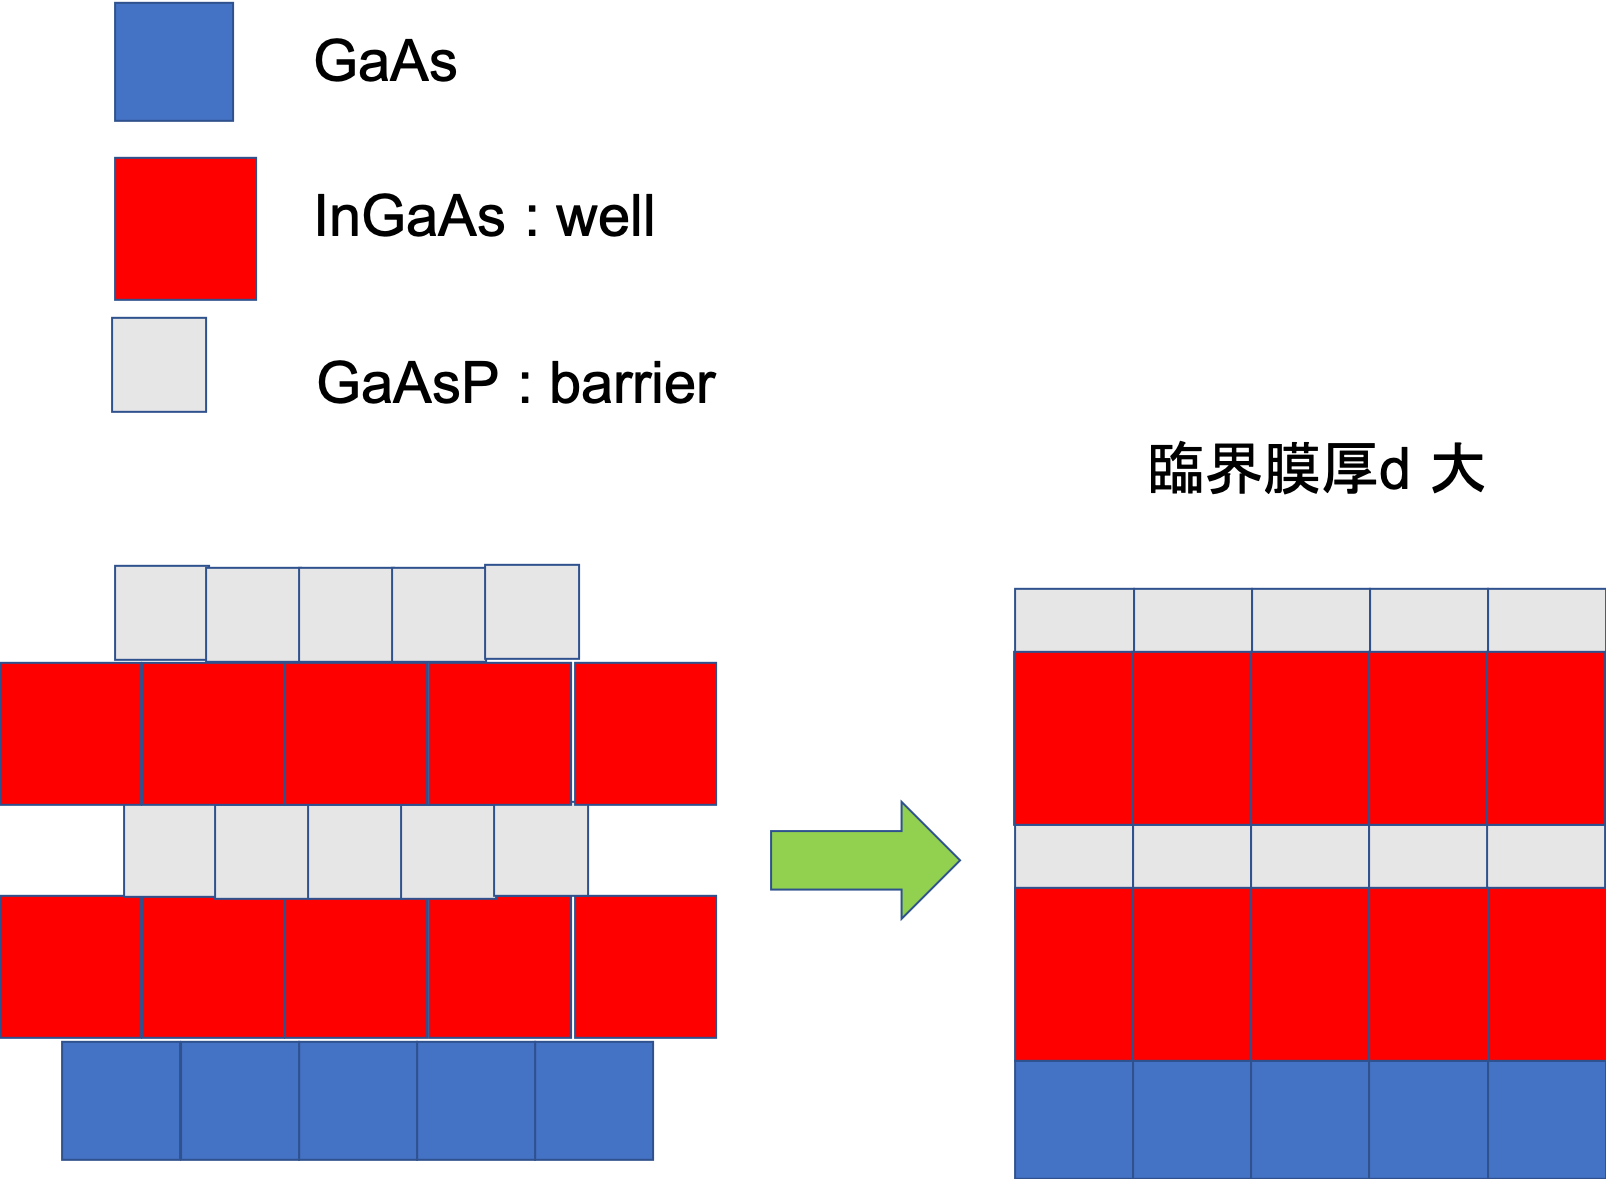
\includegraphics[width=10cm]{figure/fig_1_1_lattice_strain.png}
	\caption{格子整合の模式図}
	\label{fig:fig_1_1_lattice_strain_comp}
\end{figure}
%N.K.Duttaらは歪補償4周期InGaAs/GaAsPレーザーで$\Delta g/\Delta n =2.1 \times 10^{-15}$というそれまでのレーザーよりも高い値を報告している。また。歪み補償があるものとないもので変調感度が3dB低下する周波数が似た構造のレーザーでそれぞれ32GHz、35GHzと報告している。
%もしかして10周期ってめっちゃ多い?

\section{本研究の目的}
\begin{comment}
電流注入による直接変調を利用した利得スイッチングは従来より超短パルス発生の手法として用いられてきた。レート方程式により利得スイッチングパルスのメカニズムが説明され、短パルス化の要因として共振器長Lを短くし共振器寿命$\tau_{p}$を短くすること、およびモード利得$\Gamma g$を大きくすることが必要であると理解されてきた。特にモード利得の増大に着目すると、量子井戸の多重化による光閉じ込め係数$\Gamma$の増大の優位性も示された。

多重量子井戸化に関しては、InGaAsを井戸層としてGaAsに格子整合を行う場合にはGaAsPが歪補償のためのバリア層として有効である。

そこで本研究では多重量子井戸InGaAs/GaAsP材料を用いたレーザーデバイスをデザイン、作製することを目的とする。さらに作製した試料に対して電流注入実験を行う。デバイスのレーザー特性、特に量子井戸の多重化によるモード利得の増大が見られるかどうかを調べる。また利得スイッチング動作を試み過去の報告に匹敵する短パルス発生が可能かを推し量ることも目的とする。
%過去の報告よりもさらに多い10周期歪補償量子井戸レーザーの作製を行いさらなる短パルス化を目指す。
\end{comment}


\addspan{\adsp02{本研究では}
応用上重要な電流注入型の1\ \si{\micro\metre}波長帯InGaAs系半導体レーザーの利得スイッチング動作に注目する。GaAs材料を用いた光励起による測定実験については以前より研究室でも研究がなされ、利得スイッチングパルスのメカニズムについて説明がされてきた。しかしInGaAs材料、電流注入については先行研究\adsp02{や}参考例が少ないため基礎物理に立ち戻って設計・計画・評価測定を行いフィードバックする必要がある。}


\addspan{利得スイッチングパルスの短パルス化は、共振器長$L$を短くし共振器寿命$\tau_{p}$を短くすること及びモード利得$\Gamma g$を大きくすることで達成されることが示された。
光閉じ込め係数$\Gamma$の増大がモード利得$\Gamma g$の増大に寄与する。}


\delsp02{特にモード利得に着目すると量子井戸の多重化による光閉じ込め係数の増大の優位性も示唆されている。}\delsp02{多重量子井戸に関して、InGaAsを井戸層としてGaAsに格子整合を行う場合はGaAsPをバリア層として用いることが有効である。}


\addspan{
\adsp02{本研究では量子井戸レーザーにおいて光閉じ込め係数$\Gamma$の増大は量子井戸の層数を増やすことで実現されることに着目し多重量子井戸半導体レーザーのデザイン及び開発を行う。InGaAs系材料の格子定数はGaAs材料の格子定数よりも大きい。そのためInGaAs系材料をGaAs基板に格子整合を行いながら、層数を多くすることは格子欠陥が生じるなどの品質低下をまねきやすい。そこでGaAsよりも格子定数の小さいGaAsPをバリア層に用いることでInGaAs/GaAsP系10周期歪補償量子井戸レーザーを作製する。}}

\adsp02{電流注入では光励起と異なり電子と正孔の密度を活性層に等しく注入できるか否かは自明ではない。よって多重量子井戸の層数を増やすことで単純に高利得化を実現できるとは限らない。比較のために歪補償を行わずに結晶成長させたInGaAs/GaAs系3周期歪量子井戸レーザーの試作も行う。}
\delsp02{本研究ではこれらのことを踏まえ、InGaAs/GaAsP多重量子井戸材料を用いたレーザーデバイスをデザイン・試作・作製することを目的とする。具体的には10周期歪補償量子井戸レーザーと3周期歪量子井戸レーザーを作製する。さらに}
\delsp02{
作製した試料に対して電流注入評価測定を行う。定常電流注入実験を通してデバイスのレーザー特性を評価し、量子井戸の多重化によるモード利得の増大の有無を調べる。}


\adsp02{レーザーデバイスの作製後、定常電流注入実験を行い閾値電流及びスロープ効率の見積もりを行う。これらの値を解析することでモード利得を算出する。10周期歪補償量子井戸レーザーと3周期歪量子井戸レーザーのモード利得を比較し、期待される量子井戸多重化の効果の有無を調べる。}

\addspan{また短パルス電流注入実験を行い利得スイッチング動作を試みる。量子井戸の多重化または共振器長を短くすることによる光パルスの短パルス化が実現されるかどうかの評価測定を行うことも目的とする。}

	%序論
% !TEX root = main.tex

\chapter{試料構造と測定方法}%================================
\section{はじめに}%========================================
本研究ではInGaAs/GaAs系多重量子井戸・ファブリーペロー型の半導体レーザーをデザインし測定を行った。本章では2.2節でそのエピ構造とデバイス化のためのプロセスについて、2.3節で測定手法について述べる。
\section{試料作製}%========================================
本研究ではInGaAs/GaAs系3周期歪量子井戸レーザーおよびInGaAs/GaAsP系10周期歪補償量子井戸レーザーを作製したした。本2.2節では結晶構造のデザインと測定するためのデバイス化について述べる。エピウエハのデザインおよび結晶成長、フォトリソグラフィー加工に関してはNTT-AT社、オプトウェル社に委託し試料を作製していただいた。この場をお借りして感謝を表する。

\subsection{試料構造}%=====================================
まずはエピウエハ構造について述べる。本研究では2種類の試料を作製した。\\
(1)InGaAs/GaAs系3周期歪量子井戸構造\\
(2)InGaAs/GaAsP系10周期歪補償量子井戸構造\\
である。それぞれのエピ構造を図\ref{fig:fig_2_1_wafer_structure}に示す。
下からnタイプGaAs基板、nタイプAlGaAsクラッド層、non-GaAs SCH層(Separate Confinement Hetero-Structure)、活性層、non-GaAs SCH層、p-InGaPエッチングストップ層、p-GaAs層、p-AlGaAsクラッド層、p-GaAsハイドープコンタクト層となっている。
バンドギャップの話して発光領域の話
活性層には(1)3周期多重量子井戸のエピウエハでは量子井戸層を$\rm{In_{0.255}Ga_{0.745}As}$、バリア層をGaAsを用いた。GaAs基板に格子整合を行った。$\rm{In_{1-x}Ga_{x}As_{y}P_{1-y}}$4元混晶の格子定数はべガードの法則
\begin{eqnarray}
a(x,y)=5.8687-0.4176x+0.1896y+0.0125xy
\end{eqnarray}
で求められる\cite{ref_iga}。これより$\rm{In_{0.255}Ga_{0.745}As}$活性層の格子定数は5.7565\AA 。GaAsバリア層の格子定数は5.6532\AA であるので、面内歪$-\Delta a/a=$は-0.0183 となる。InGaAs層に圧縮歪が生じている。(2)10周期量子井戸のエピウエハにおいては量子井戸層を同様に$\rm{In_{0.255}Ga_{0.745}As}$、バリア層では歪補償のために$\rm{GaAs_{0.71}P_{0.29}}$を用い、GaAs基板に格子整合を行った。(GaAsPのGaAsに対する歪は$-\Delta a/a=0.010$でありGaAsPには引っ張り歪が生じている)

また図\ref{fig:fig_2_1_wafer_structure}にはバンドギャップ$E_{g}$と屈折率nの変化を模式的に表した。光は活性層とSCH層、p-InGaAs層、p-GaAs層に閉じ込められると考えいている。またキャリアは$E_{g}$の小さい量子井戸へ流れ込む。量子井戸で再結合がおこる。

エピウエハ完成後フォトリソグラフィによって電極パターンを形成した。それについて次節で述べていく。
\begin{figure}[h]
	\centering
	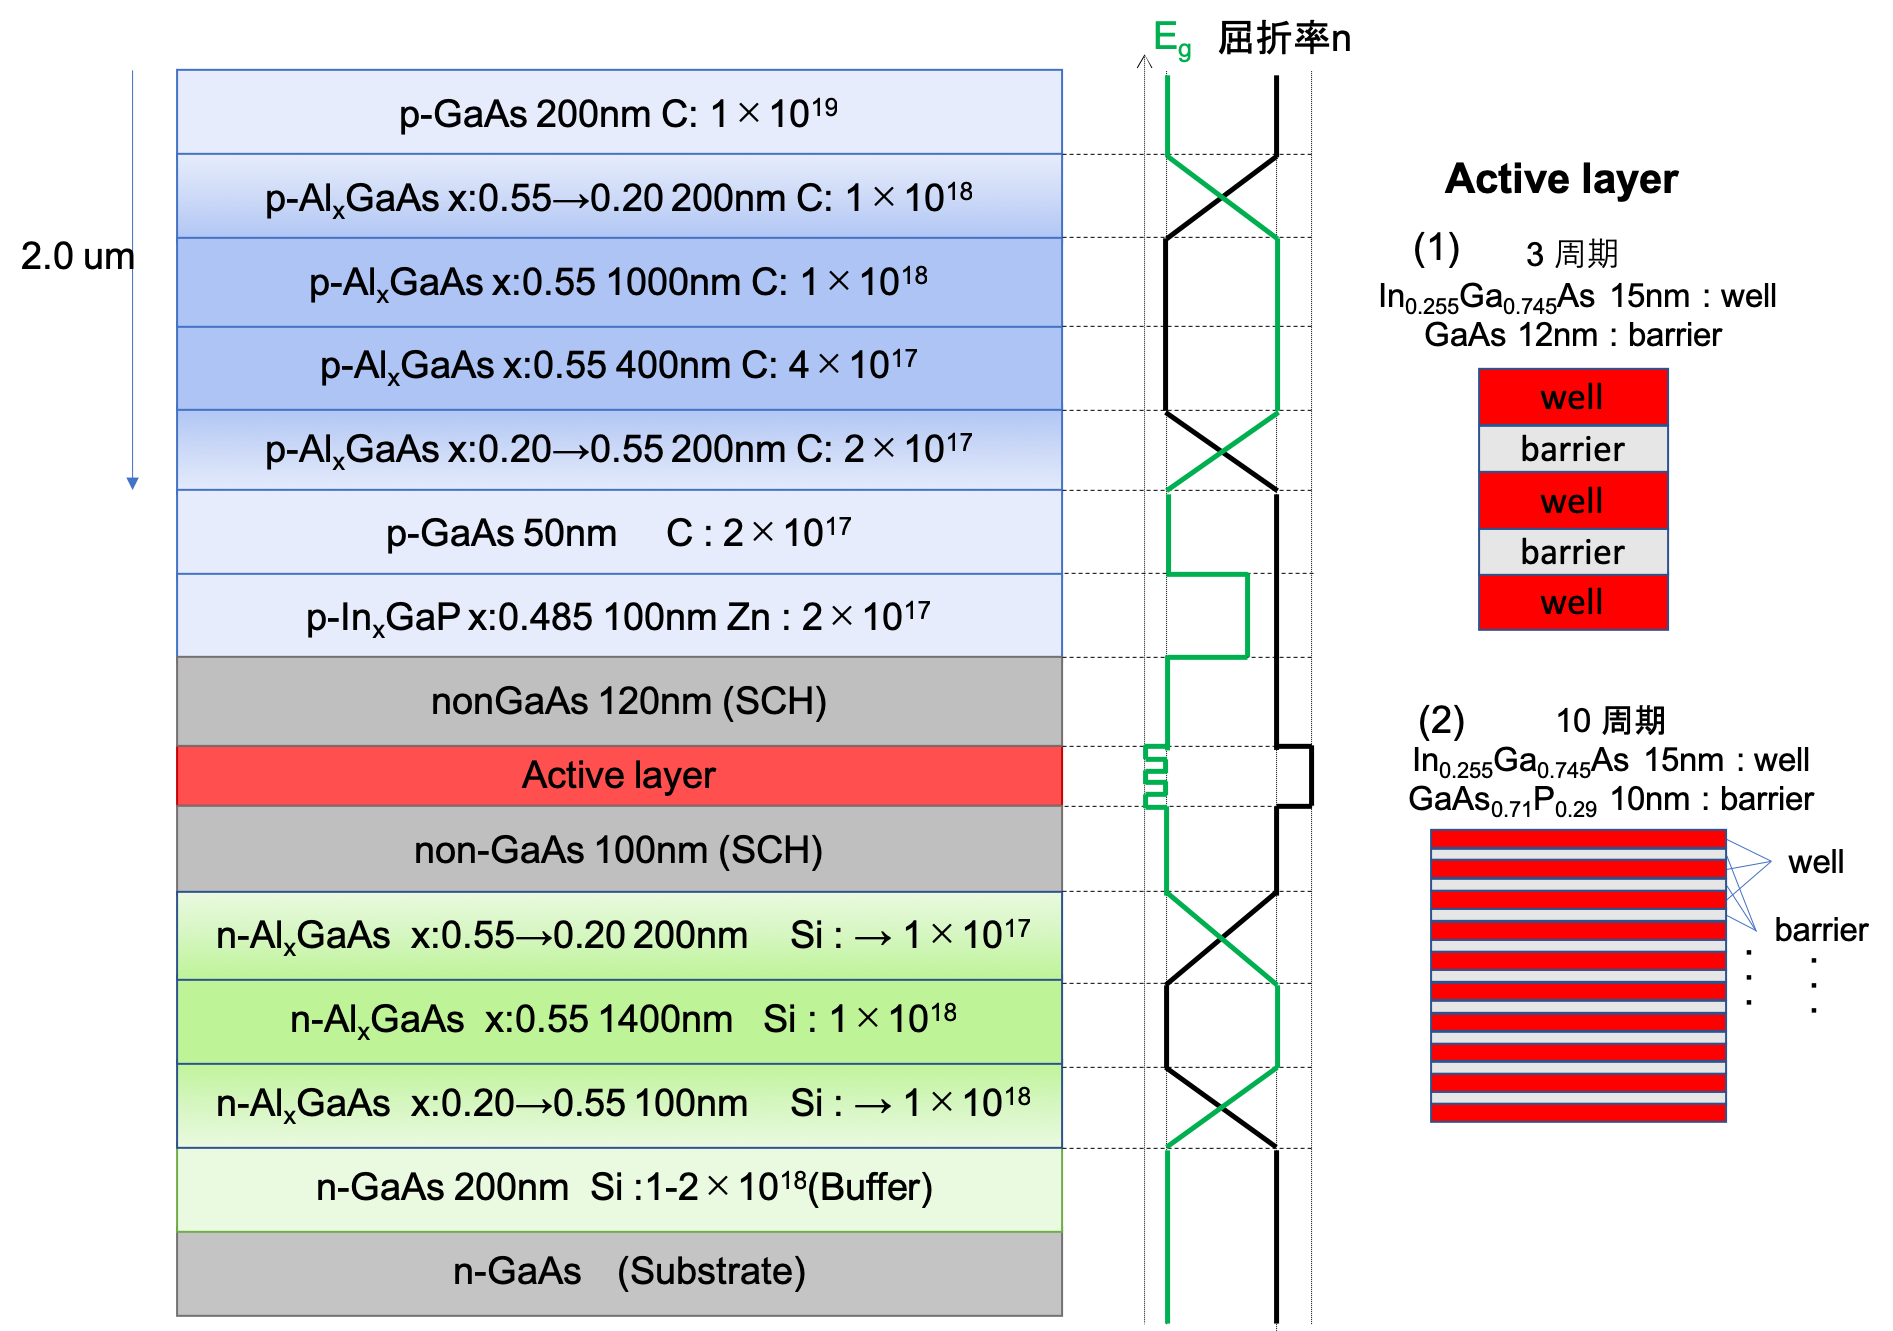
\includegraphics[width=10cm]{figure/fig_2_1_wafer_structure}
	\caption{エピウエハ構造}
	\label{fig:fig_2_1_wafer_structure}
\end{figure}
%\clearpage
\subsection{ブロードコンタクトレーザー}%=======================
ブロードコンタクトレーザーとは光導波路を形成せずコンタクト電極をベタに蒸着したレーザーデバイスである。リッジ形成プロセスを簡略化することで早く測定を行うことを目的とした。ウエハの評価測定のために用いた。
エピウエハのn側とp側にコンタクトメタルの蒸着を行った。p側の原子はAuZnNiをコンタクトメタルとしTi/AuおよびAu電極を使用した。基板を研磨し120um厚とした。その後n側はAuGeNiを用いて電極を蒸着した。


劈開を行いレーザーデバイス化した後の模式図を図\ref{fig:sample_broadcontact}に示す。z方向にファブリーペロー共振器が形成される。y方向に電流が流れ、活性層でキャリアの再結合が起きる。赤い楕円で示した。注入キャリアの量が閾値を超えると反転分布となり誘導放出がおこる。光が共振器内部を往復することで増幅され発振に至る。

共振器長はL=500,1000,2000umの3種類を作製した。
x方向の電流の広がりの大きさを定める電極の幅を「電極パッド幅w」と呼ぶことにする。電極パッド幅はw=3,5,10,30,50,100,300umの6種類を作製した。

\begin{figure}[h]
	\centering
	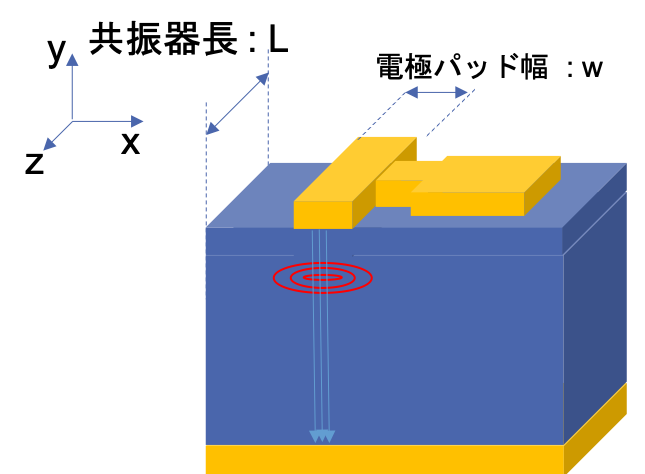
\includegraphics[width=8cm]{figure/fig_2_1_broadcontact.png}
	\caption{ブロードコンタクレーザー}
	\label{fig:sample_broadcontact}
\end{figure}

\subsection{リッジ導波路型レーザー}%==========================
次にリッジ導波路型レーザーについて述べる。その模式図を図\ref{fig_2_1_ridge}に示す。エピウエハ作製後p側クラッド層をy方向に活性層直上までエッチングすることで光導波路を形成した。そのときx方向のリッジ幅をwと呼ぶ。x方向の光閉じ込めが大きくなるため、キャリアと光の重なりが大きくなることにより利得を大きくすることができる。%参考文献ほしい
商用デバイスにおいても一般的に行われている手法である。本研究でも最終的に利得スイッチング動作をこれらの試料に対して試みた。

導波路リッジの深さは3周期試料は実測値で1.8um、10周期試料は1.9$\sim$2.0umである。導波路リッジ幅はw=1.5um,2.5umのものを作製した。
AuZnNiをコンタクトメタルとしてTi/Auを電極とした。
基板を研磨し120um厚とした。n側コンタクトはAuGeNi/Auである。
共振器長L=100,200,300,400,500,1000umに劈開を行った。共振器長が100,200umのものは劈開の真っ直ぐさを保つために60um厚と非常に薄く研磨した。
\begin{figure}[h]
	\centering
	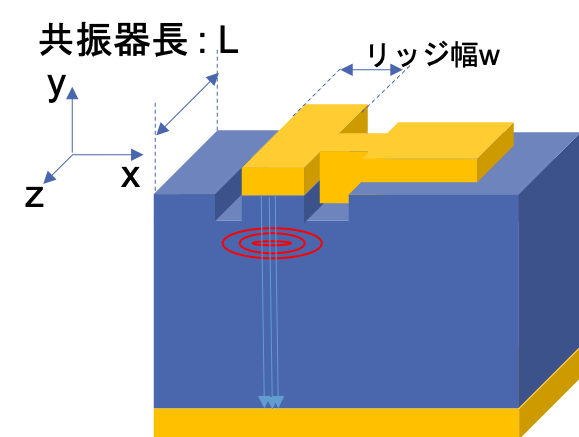
\includegraphics[width=8cm]{figure/fig_2_1_ridge.png}
	\caption{リッジ導波路型レーザー}
	\label{fig_2_1_ridge}
\end{figure}

\subsection{マウント}%======================
作製したブロードコンタクトレーザーおよびリッジ導波路型レーザーに電流注入実験を行うためにマウントを行なった。
同じエピウエハから切り出したレーザー試料でも、行う測定によって適したマウントの仕方に変えている。


定常電流を流す実験を行うためにマウントした試料の例を図\ref{fig:fig_2_1_mount}(a)に示す。写真中心の青い棒状のものがレーザーデバイス(レーザーバー)であり、合計5つの異なる電極パッドがついている。z方向の共振器長は300umである。誘導放出光はz方向に放射する。レーザーバーの下にあるオレンジ色の部分がAlN基板の全面にAnSnメッキを施したサブマウント(京セラ社製)である。AlNサブマウントの大きさは2cm×5mmであり、試料の取り扱いを平易にするためにダイボンディングを行った。ダイボンディングはAnSuの融点よりも高い330℃まで加熱したサブマウントの上にレーザーバーを吸引ピンセットでおいた。レーザの端面をAlNサブマウントの淵に合わせることが後の測定で光検出器を近づけるために大事である。このときAnSuの酸化を防ぐために$N_{2}$雰囲気下で行った。
%ブロードコンタクトレーザーはダイボンディングしてなかったっけ?そういえば


ダイボンディングが終わった試料はxzyステージに置いて測定を行った。試料上面のp側電極をプローバー
%(先端の径...程度の金属の針)
でさわり電流を流した。n側はAuSnメッキAlNサブマウントを銅板などの導体に置き、その銅板から配線を行った。1本のレーザーバーに5から6個程度の電極素子があるため1つの素子に対して測定が終わると次々とプローバーさわる箇所をかえていった。そうすることで速やかに測定を続けることができる。


 一方、利得スイッチング動作実験(高周波電気パルスを駆動)を行う試料は短い電気パルスが入るようにTransistor Outlineパッケージと呼ばれる缶状の金属にマウントを行った。京セラ社製のCANを用いた。レーザーバーからさらに切り出された1つ1つに分離した素子をAnSn共晶材あるいはエポキシを用いてTO-CANにダイボンディングし、p側電極には金線をワイヤーボンディングマシンで配線した。その例を図\ref{fig:fig_2_1_mount}(b)に示す。図\ref{fig:fig_2_1_mount}(b)の上段の写真は1つのレーザー素子(1つの電極)がTO-CANに乗せられた状態を上から(y軸方向から)みた様子を示している。縮小したものと拡大したもの2種類の写真である。また図\ref{fig:fig_2_1_mount}(b)の下段には同じ試料をz方向からみた図を示す。レーザーの端面と金線がブリッジ状に配線されている様子が見える。

CANタイプの試料は専用の治具を作製しxyzステージに固定して測定を行った。固定したのちCANの後ろから出ている足に同軸ケーブルのプラス側とマイナス側をそれぞれ配線して回路を作製した。

\begin{figure}[h]%測定デバイス外観
	\centering
	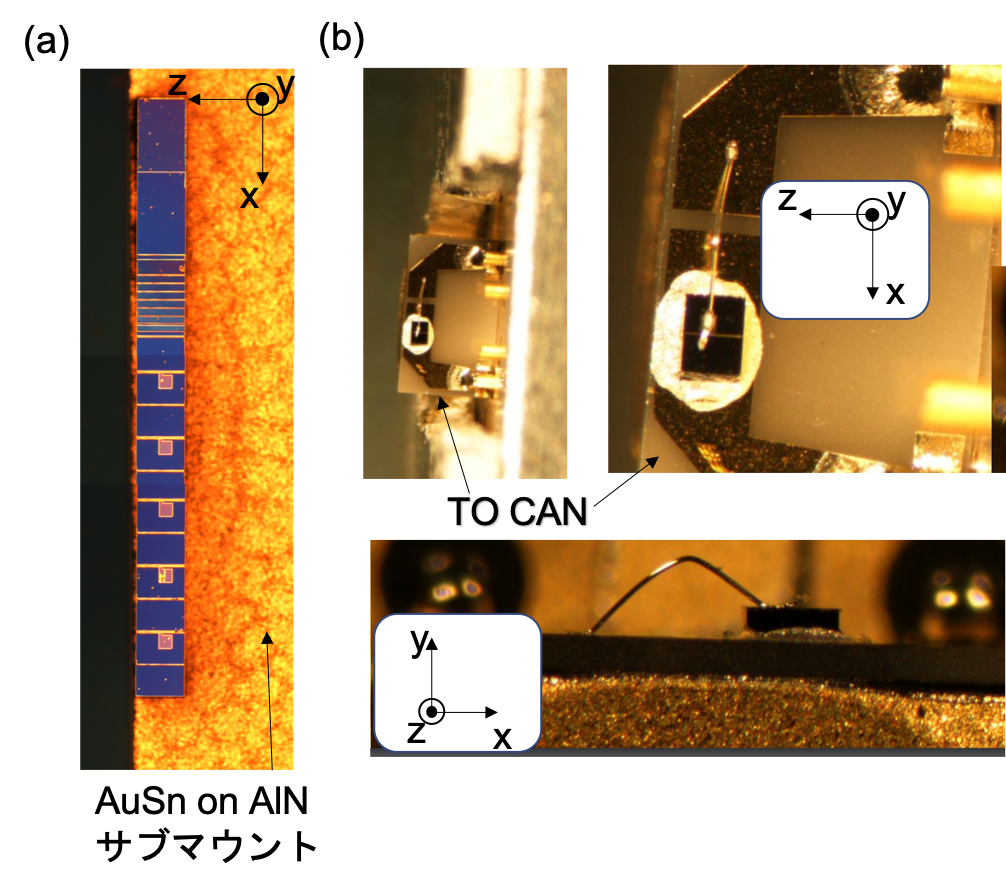
\includegraphics[width=15cm]{figure/fig_2_1_mount.png}
	\caption{測定デバイス外観}
	\label{fig:fig_2_1_mount}
\end{figure}

\clearpage
\section{測定方法}%========================================
本研究では2つの実験を行った。1つはエピウエハの品質を評価するための定常電流を印加する実験である。もう一つは利得スイッチング動作を起こすための短い電気パルスを印加する実験である。それぞれについて2.3.1節と2.3.2節で述べる。
\subsection{定常電流注入による測定実験}%=======================
まずエピウエハの品質を調べるために定常電流を注入する実験について述べる。発振閾値電流や発振時の発光効率すなわち外部量子効率などの基本的な物性パラメータを見積もることを目的として行った。
実験系の回路図を図\ref{fig:fig_2_2_IL_setup}に示す。パルスジェネレータから数usパルスを数ms繰り返し周期で発生させ試料に注入する。ここでマイクロ秒程度のパルスは試料の中での発光過程やその他の高速な物理現象の時間オーダーに対して十分長く、その間に定常発振しているとみなした。DC電流では熱の影響が大きくなってしまい試料が壊れてしまう恐れがあるため。Duty比(パルス幅と繰り返し周期の比)を1:1000程度に設定して実験を行った。試料からの発光強度を光パワーメータで測定した。また、回路に試料と直列に抵抗(22.4$\rm{\Omega}$)を入れ、そこにかかる電圧をモニタすることで流れる電流を見積もった。回路全体の電圧と抵抗にかかる電圧の差をとることで試料にかかる電圧を算出した。
試料はレーザーバー状になっているものを測定した。レーザーバーは銅板の上に置かれ、銅板はペルチェ素子および温度コントローラで25℃に温度調節した。

\begin{figure}[htbp]
	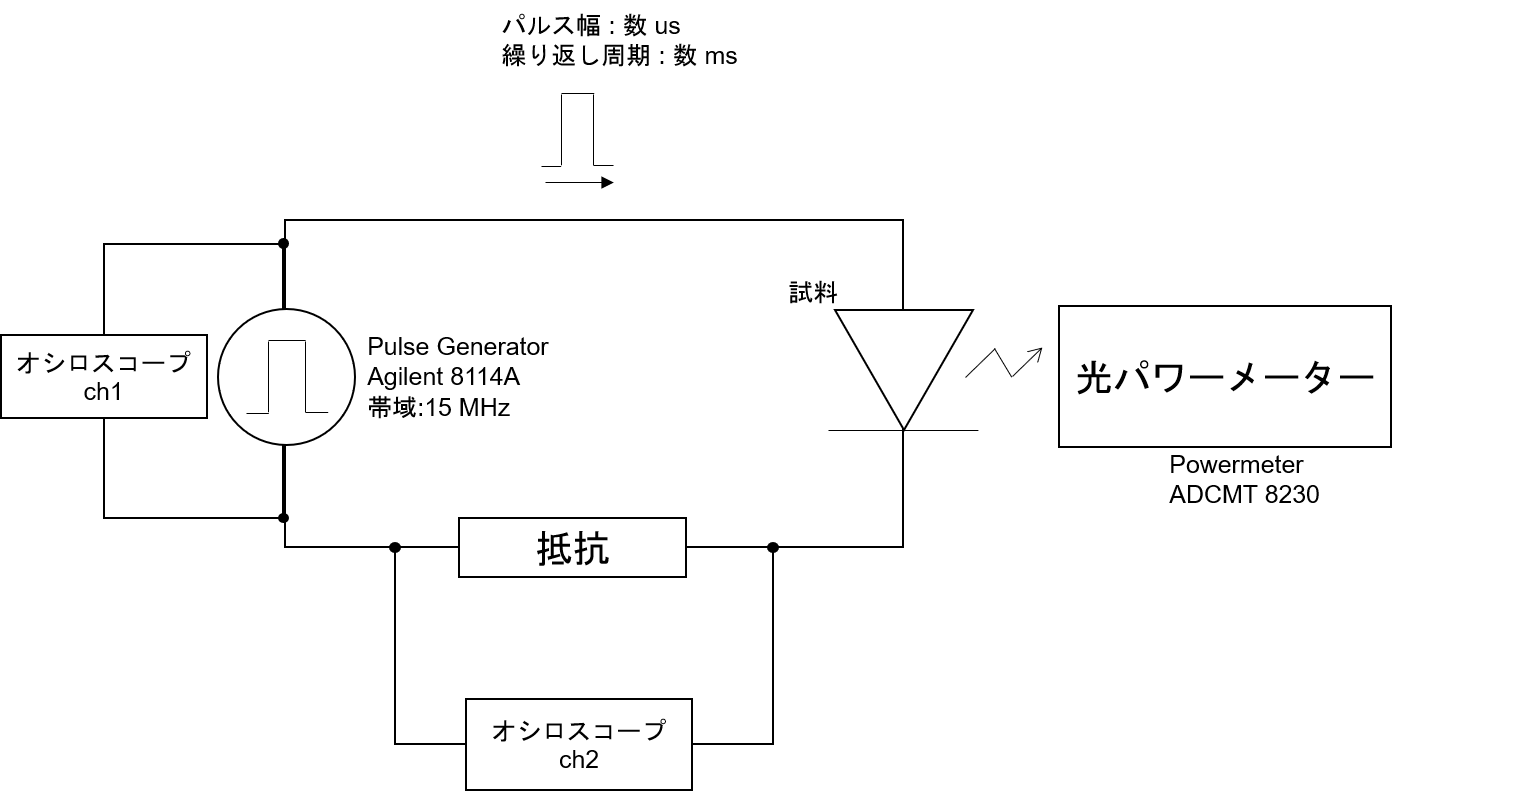
\includegraphics[width=15cm]{figure/fig_2_2_IL_setup.png}
	\caption{定常電流注入実験の実験系回路図}
	\label{fig:fig_2_2_IL_setup}
\end{figure}
\clearpage
ここで用いた機材を\ref{table:table_2_2_IL_setup}に示す。
\begin{table}[h]
  \caption{定常電流印加実験に用いた機材}
    \label{table:table_2_2_IL_setup}
  \centering
  \begin{tabular}{lccc}
    \hline
    機材  & 型番 &帯域  & その他  \\
    \hline \hline
    Pulse Generator  & Agilent 8114A & 15MHz &最大50V \\
    Power Meter  &  ADCMT 8230 & -&-  \\
    Oscilloscope  &  Agilent DSO5054A &500MHz&- \\
    Temperture Controller & ILX Lightwave  LDT5412&-\\
       \hline
  \end{tabular}
\end{table}
\subsection{電流注入利得スイッチング実験}%======================
次にナノ秒程度の短いパルス電圧を印加する実験について述べる。利得スイッチング動作を起こしその光パルスの時間波形を取得しパルス幅を見積もることを目的とした。

短パルス印可の実験にはCANタイプの試料を用いた。CANは専用の治具に固定されxyzステージに乗せて測定した。治具にはペルチェ素子がついており温度コントローラーで25℃に調節した。


実験系の模式図を図\ref{fig:fig_2_3_GS_setup}に示す。1ns電気パルスがパルスジェネレータから発生され、可変抵抗のAttenuatorを通り、RFアンプで増幅されデバイスへと印可される。回路は全て同軸ケーブルを用いており50$\Omega$のインピーダンスマッチをとった。

試料からの発光はNA=0.5の対物レンズでコリメートされ、焦点距離13.86mm、NA=0.18の非球面レンズで光ファイバーに集光される。光学系素子は半導体端面からの発光の広がり、光ファイバーのNAに合わせたものを使用した。光ファイバーを通した光はフォトダイオードで検出され、その電圧を高速サンプリングオシロスコープでモニタすることで光の時間波形を測定した。
\begin{figure}[h]
	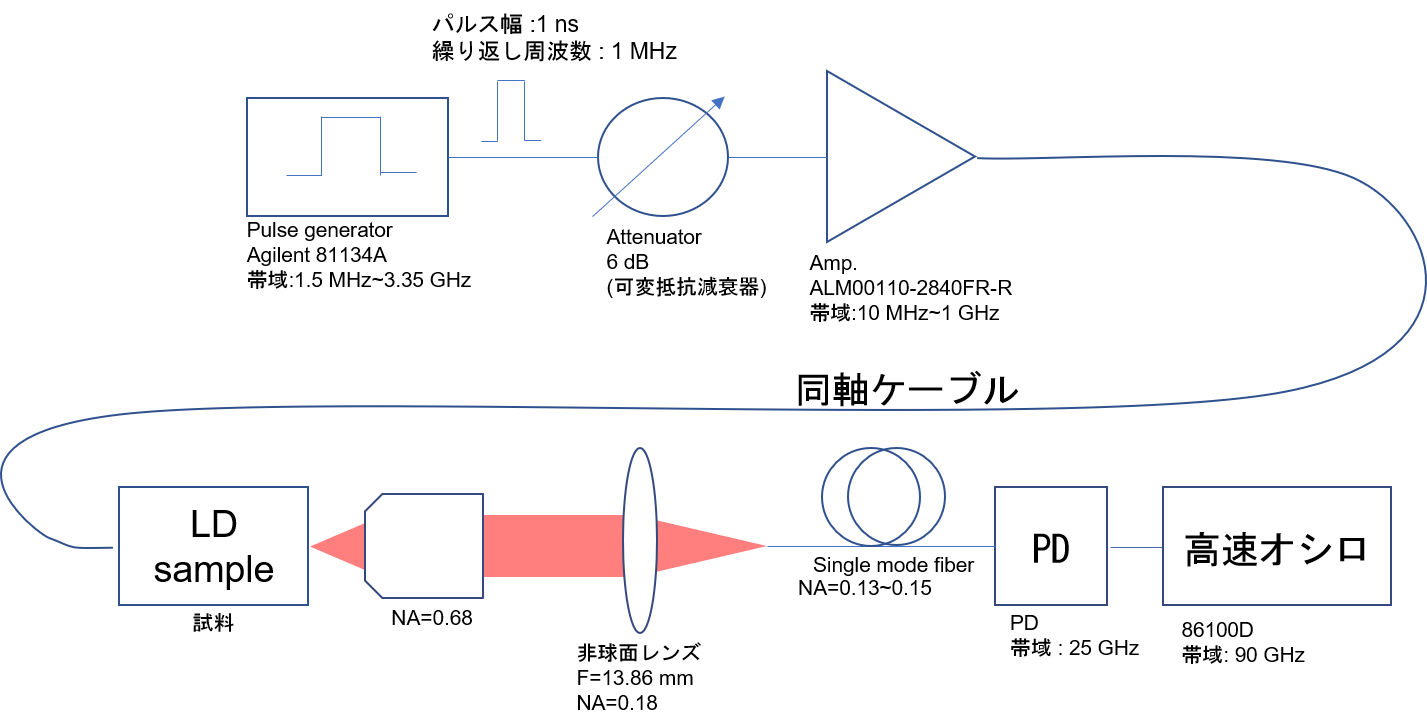
\includegraphics[width=15cm]{figure/fig_2_3_GS_setup.png}
	\caption{GS実験系}
	\label{fig:fig_2_3_GS_setup}
\end{figure}


この実験で用いた機材を表\ref{table:table_2_2_GS_setup}にまとめた。
\begin{table}[h]
  \caption{利得スイッチング実験に用いた機材}
  \label{table:table_2_2_GS_setup}
  \centering
  \begin{tabular}{cccc}
    \hline
    機材  & 型番   & 周波数帯域 &電圧 \\
    \hline \hline
    Pulse Generator  & Agilent 81143A & 1.5MHz$\sim$ 3.35GHz  &最大2V \\
    Atteuator  &  Aeroflex/Weinschel model 940-60-11    & DC $\sim$4.0GHz& -6dB$\sim$ -66dB\\
    RF Amp & ALM00110-2840FR-R & 10MHz $\sim$ 1GHz & +28dB\\
    PD & New Focus model 1414 & 25GHz &-\\
    Oscilloscope  &  Keysight 86100D & 90GHz  &-\\
     Temperture Controller & ILX Lightwave  LDT5412&-&-\\
       \hline
  \end{tabular}
\end{table}
		%試料構造と測定方法
\chapter{実験結果}
\section{ブロードコンタクトレーザーバー試料に関する測定結果}%=====================================
ブロードコンタクトレーザーバーに関してはウエハの特性を調べるために定常電流を流して測定を行なった。熱の発生を抑制するためにパルス電流を用いた。電流は...ms秒周期、...μsのパルス電流を流した。μs程度の電流は試料にとっては定常と見なされる。
まずは定常状態の測定。発振閾値電流を測定することに加えて、発振時の印可電流の増分したいする光出力の増大から発光量子効率を見積もることが目的である。
様々なパラメータを測定する。ウエハの構造ごとに節を分けている。
\subsection{3QW}%===============================
\begin{figure}[h]
	\centering
	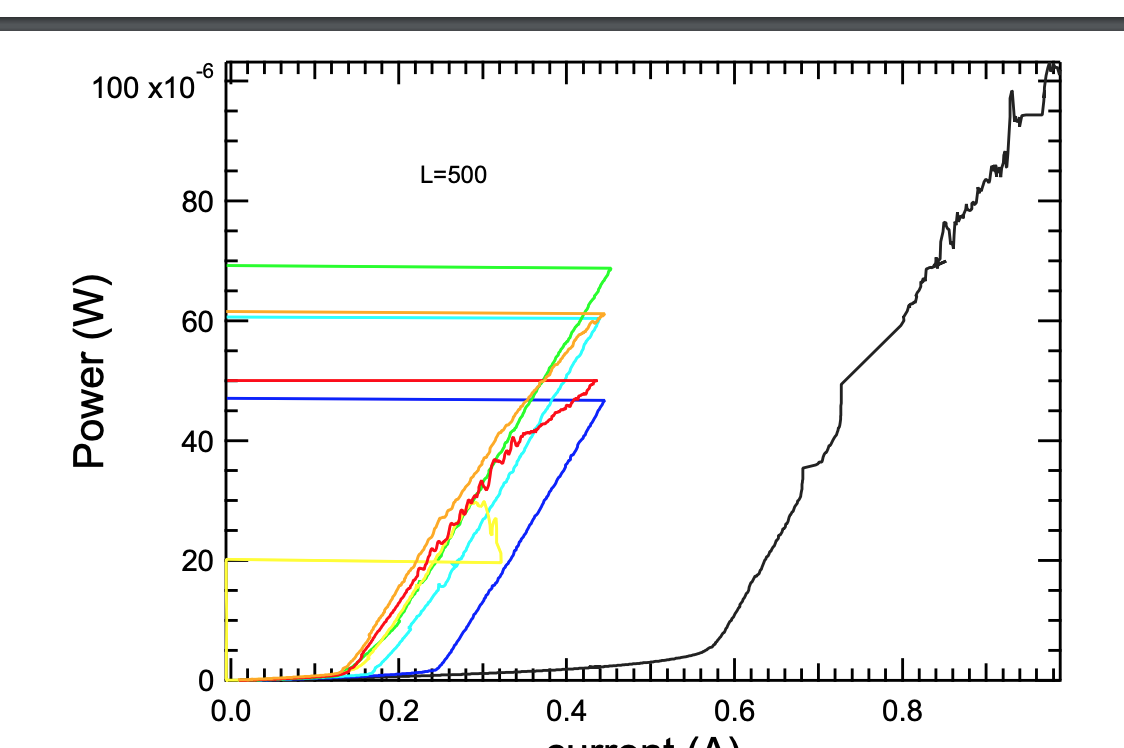
\includegraphics[width=10cm]{figure/fig_3_1_IL_broad_3QW.png}
		\caption{3MQWのIL結果}
		\label{fig_3_1_IL_3QW.png}
\end{figure}
閾値の表この表違うかも
\begin{table}[hbtp]
  \caption{閾値}
  \label{table:data_type}
  \centering
  \begin{tabular}{lcr}
    \hline
    共振器長  & 宣言  &  ビット幅  \\
    \hline \hline
    文字型  & char  & 8 \\
    整数型  & int   & 32 \\
    倍精度実数型  & double  & 64 \\
    倍々精度実数型  &  long double  &  96 \\
    \hline
  \end{tabular}
\end{table}

\begin{figure}[h]
	\centering
	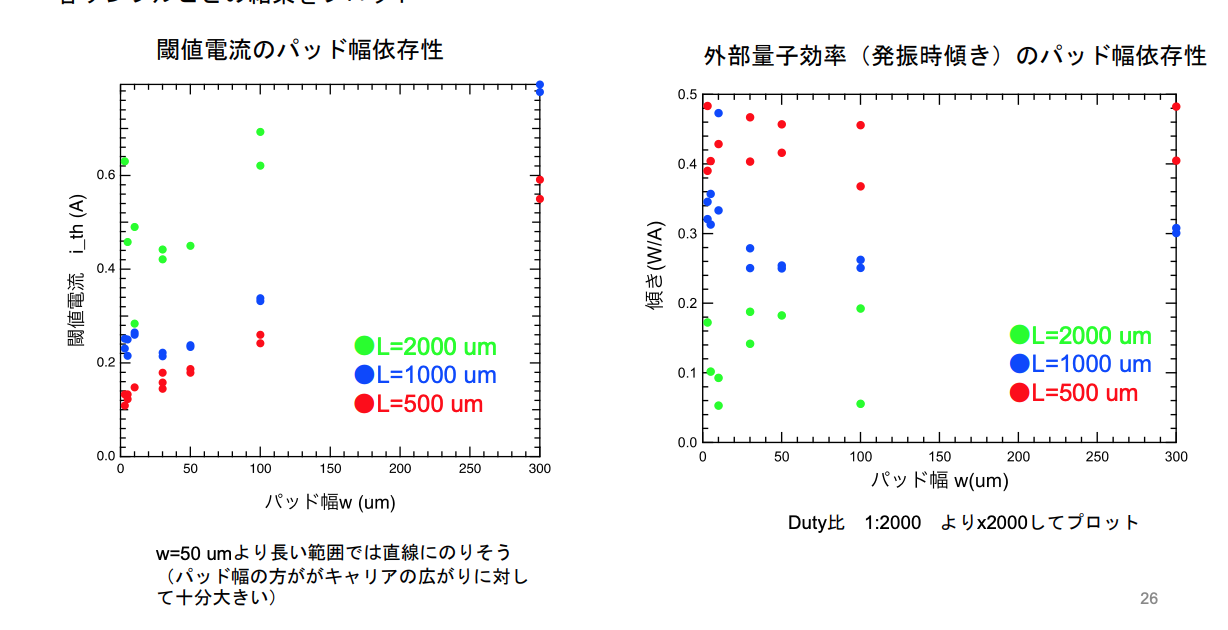
\includegraphics[width=10cm]{figure/fig_3_1_broad_i_th_3QW.png}
		\caption{3MQWの閾値電流}
		\label{fig_3_1_broad_i_th_3QW}
\end{figure}

\begin{figure}[h]
	\centering
	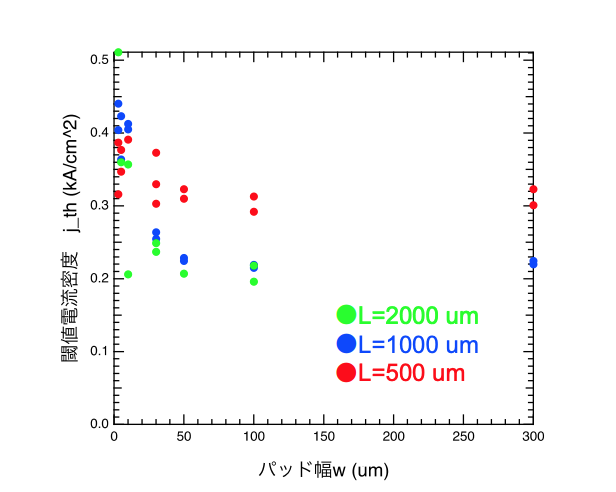
\includegraphics[width=10cm]{figure/fig_3_1_broad_j_th_3QW.png}
		\caption{3MQWの閾値電流密度のパッド幅依存性}
		\label{fig_3_1_broad_j_th_3QW}
\end{figure}

\newpage
\subsection{10QW}%===============================
\begin{figure}[h]
	\centering
	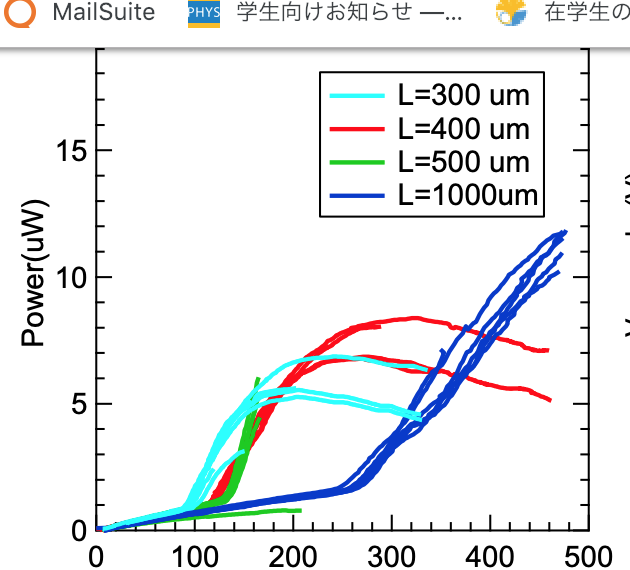
\includegraphics[width=10cm]{figure/fig_3_1_IL_10QW.png}
		\caption{10MQWのIL結果}
		\label{fig_3_1_IL_10QW.png}
\end{figure}
\begin{figure}[h]
	\centering
	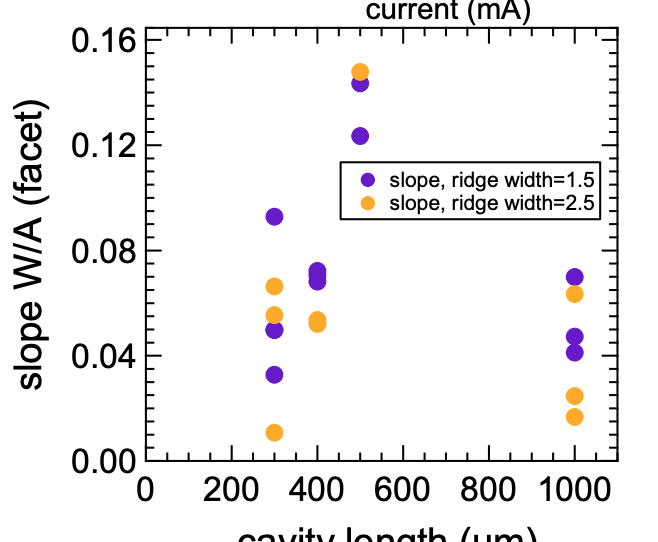
\includegraphics[width=10cm]{figure/fig_3_1_broad_slope_10QW.png}
		\caption{10MQWのスロープ}
		\label{fig_3_1_IL_broad_slope}
\end{figure}
閾値の表この表違うかも
\begin{table}[hbtp]
  \caption{閾値}
  \label{table:data_type}
  \centering
  \begin{tabular}{lcr}
    \hline
    共振器長  & 宣言  &  ビット幅  \\
    \hline \hline
    文字型  & char  & 8 \\
    整数型  & int   & 32 \\
    倍精度実数型  & double  & 64 \\
    倍々精度実数型  &  long double  &  96 \\
    \hline
  \end{tabular}
\end{table}

\begin{figure}[h]
	\centering
	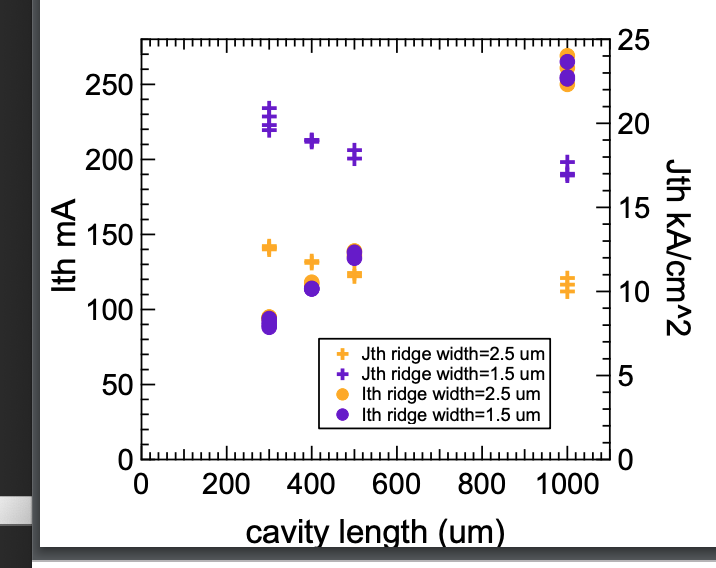
\includegraphics[width=10cm]{figure/fig_3_1_broad_i_th_10QW.png}
		\caption{10MQWの閾値電流}
		\label{fig_3_1_broad_i_th_3QW}
\end{figure}

\begin{figure}[h]
	\centering
	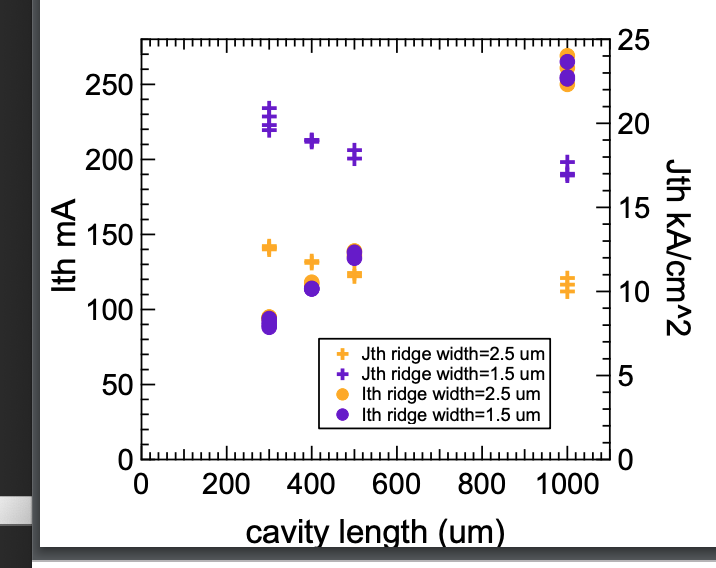
\includegraphics[width=10cm]{figure/fig_3_1_broad_i_th_10QW.png}
		\caption{10MQWの閾値電流密度のパッド幅依存性}
		\label{fig_3_1_broad_j_th_10QW}
\end{figure}

\newpage
\subsection{内部量子効率と吸収係数の計算}%=============
\begin{figure}[htbp]
	\centering
	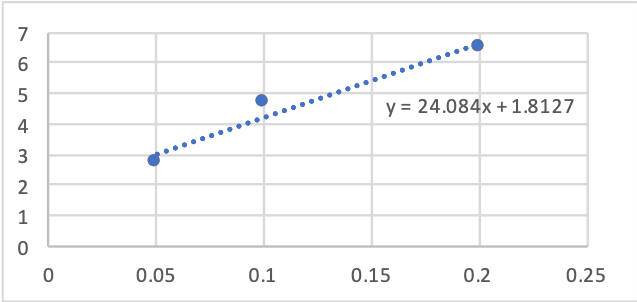
\includegraphics[width=10cm]{figure/fig_efficientcy_vs_L_inverce.png}
	\caption{外部量子効率 対共振器長の逆数}
	\label{fig:efficientcy_vs_L_inverce}
\end{figure}
\begin{figure}[h]
	\centering
	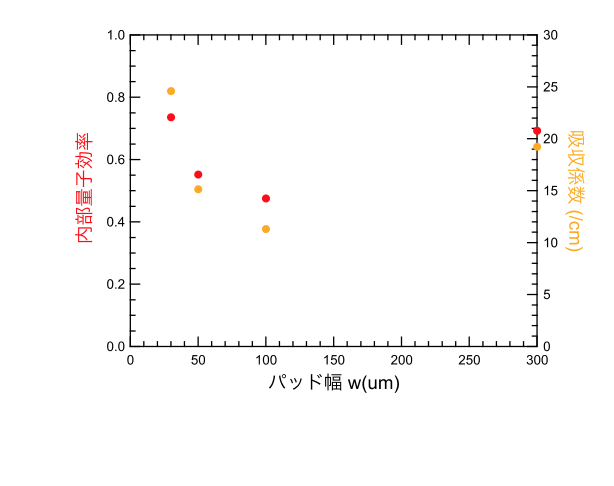
\includegraphics[width=10cm]{figure/fig_3_1_eff_in_3QW.png}
		\caption{3MQWのIL結果}
		\label{fig_3_1_IL_broad_i_th_3QW}
\end{figure}
\subsection{電流広がりに関する考察}%==================

\newpage
\newpage
\newpage
\section{電流注入利得スイッチング}%===================
リッジ導波路型レーザーに関して電流注入利得スイッチング実験を行った。その結果を示す。
\subsection{3QW}%===============================

\subsection{10QW}%==============================


		%実験結果
%\chapter{考察}
\label{chap:simulation}

\section{はじめに}

\section{パルス幅と共振器長の関係}	%考察
% !TEX root = main.tex

\chapter{まとめと展望}
この章では本研究で得られた結論と展望について述べる。
\section{本研究のまとめ}%InGaAs系高利得半導体レーザーの開発および評価測定
利得スイッチングパルスの短パルス化はモード利得を大きくすることと共振器寿命を短くすることで達成され得ることが示されていた。本研究では利得層を厚く積むことにより高利得化を意図した多重量子井戸レーザー作製すること、また作製したデバイスの特性を測定することを目的とした。レーザー試料作製を行い定常電流および短パルス電流を注入する実験を行った。

%1\si{\micro\metre}帯の
GaAsに対して格子定数が大きいInGaAs材料を厚く積層するためにバリア層に格子定数の小さいInGaPを用いた10周期歪補償量子井戸構造ウエハを作製した。また比較のために3周期歪量子井戸構造のウエハも作製した。エピウエハをデバイス化しブロードコンタクトレーザーとリッジ導波路型レーザーを作製した。マウントを行い電流注入実験を行った。

ブロードコンタクトレーザーに対して定常電流注入実験を行ったところ
%高い抵抗値と
電流が流れる幅を決める電極パッド幅に対して優位にが広がっていることがわかった。広がりは3周期歪量子井戸試料では60 \si{\micro\metre}程度
、10周期歪補償量子井戸試料では25$\sim$50 \si{\micro\metre}と見積もられた。閾値電流密度を見積もると3周期歪量子井戸レーザーでは0.20$\sim$0.35 $\rm{kA/cm^{2}}$、10周期歪補償量子井戸レーザーでは0.40 $\rm{kA/cm^2}$と見積もられた。また透明電流密度と微分利得係数の比はそれぞれ4.6倍、3.7倍と見積もられ多重量子井戸化の効果をみることができた。

リッジ導波路型レーザーについて定常電流注入実験を行ったところ。10周期歪補償量子井戸レーザーに関して発光量の減衰が観測された。追加実験により原因が特定できると考えられる。


リッジ導波路型レーザーについて短パルス注入実験を行った。3周期歪量子井戸レーザーについてはインピーダンス不整合のために典型的な利得スイッチングパルスをみることが困難であったが最短のパルス幅として28.9 psを得た。また10周期歪補償量子井戸レーザーに関しては典型的な利得スイッチングパルスを観測することができ、最短パルス幅は26.5psであった。

モード利得あるいは共振器長の違いによるパルス幅の差異は明確ではなかった。この原因として電気信号の帯域による制限がかけられているものと考えられる。

\section{今後の展望}
3周期歪量子井戸レーザーと10周期歪補償量子井戸レーザーで比較したときモード利得の増大が見られた。エピウエハデザインの段階で期待した効果が見えた。一方でInGaP層によるキャリア広がりも観測された。このことからInGaP層の薄い構造のデバイスを作製することがより高品質なレーザーを開発する上で肝心となるのではないかという知見を得た。


電流注入利得スイッチング実験についてはパルス幅は電気パルスの帯域制限を受けていると考えられるため駆動系の改善を行いたい。十分短い電気パルスで強く励起した場合にこそ高利得化の利点が見られと考えられる。	%まとめと展望

\chapter{付録}

%\section{deconvolutionの計算}
%\section{駆動系の電気信号}
%\section{GaAsの発振}
%線形離島の領域なの?
\section{格子定数、$E_{g}$の計算}
$\rm{In_{1-x}Ga_{x}As_{y}P_{1-x}}$の格子状数は\cite{ref_iga}より
\begin{eqnarray}
a=5.8687-0.4176x+0.1896y+0.0125xy\\
\end{eqnarray}
と計算した。$\rm{Al_{1-x}Ga{x}As}$の格子定数は
\begin{eqnarray}
a=5.65325x+5.6605(1-x)
\end{eqnarray}
として計算した。
$E_{g}$は下の表の式を用いて計算を行った。
\begin{table}[h]
  \caption{3周期歪量子井戸ブロードコンタクトレーザーの電流広がり}
  \label{table:table_Eg}
  \centering
  \begin{tabular}{cc}
    \hline
    材料& $E_{g}$の式   \\
    \hline \hline
     $\rm{Ga_{x}In_{1-x}As}$ &$0.324+0.7x+0.4x^2$   \\
    $\rm{Al_{x}Ga_{1-x}As}$& $1.420+1.087x+0.438x^2$ \\
    $\rm{Ga_{x}In_{1-x}P}$& $1.351+0.643x+0.786x^2$ \\ 
    $\rm{GaAs_{x}P_{1-x}}$&$2.750-1.502x+0.176x^2$\\
    \hline
  \end{tabular}
\end{table}
%\subsection{InGaPのトンネル}

 		%付録
%% reference
% !TEX root = main.tex
\begin{thebibliography}{99}
%1
\bibitem{ref_hasegawa} A. Hasegawa and Y.Kodama, Signal transmission by optical solitons in monomode fiber, \sl Proc. IEEE\rm ,vol.69, No.9, 1145-1150, 1981.
%2
\bibitem{ref_chichkov} B.N. Chichkov, C.momma, S.Nolte,F. von Alvensleben, A. T$\rm{\ddot{u}}$nnermann, Femtosecond, picosecond and nanosecond laser ablation of solids. \sl Appl. Phys. A\rm vol.63,109-115, 1996.
%3
\bibitem{ref_h_ito} Hiromasa Ito, Shigeru 
murata, Hiroyuki Yokoyama and Humio Inaba. 高周波変調にもとづくAlGaAs半導体レーザーからの超短光パルス発生, 応用物理, 第50巻, 第1号, 18-28, (1981).
%4
\bibitem{ref_aspin} G.J. Aspin ,J.E.Carroll,and R. G. Plumb . The effect of cavity lenght on picosecond pulse generation with highly rf modulated AlGaAs double heterostructure lasers. \sl Appl. Phys. Lett\rm , Vol. 39, p. 860, 1981.
%5
\bibitem{ref_torphammar} P. Torphammar, S. T. ENG. PICOSECOND PULSE GENERATION IN SEMICONDUCTOR LASERS USING RESONANCE OSCILLATION. \sl ELECTRONICS LETTERS\rm , vol. 16, No. 15, p. 587, 1980.
%6
\bibitem{ref_nagarajan} Radhakrishan Nagarajan, Takeshi Kamiya, Akihiko Kasukawa, and Hiroshi Okamoto. Observation of ultrashort($< $4 ps) gain-switched pulses from long-wavelength multiple quantum well lasers. \sl Appl. Phys. Lett.\rm , Vol. 55, p. 1273, 1989.
%7
\bibitem{chen_yokoyama} Shaoqiang Chen, Aya Sato, Takashi Ito, Masahiro Yoshita, Hidefumi Akiyama, and Hiroyuki Yokoyama. Sub-5-ps optical generation from a 1.55 \si{\micro\metre} distributed-feedback laser with nanosecond electric pulse exitation and spectral filtering. \sl Optics Express\rm , Vol.20, No.22, 2012.
%8
\bibitem{ref_h_yokoyama} Hiroyuki Yokoyama, Hengchang Guo , Takuya Yoda, Keijiro Takashima, Ki-Ichi SaTo, Hirokazu, Taniguchi, anc Hiromasa Ito, Two-photon bioimaging with picosecond optical pulses from a semiconductor laser,\sl OPTICS EXPRESS\rm , vol. 14, No.8,2006.
%8
\bibitem {ref_lau} K. Y. Lau. Gain switching of semiconductor Injection lasers, \sl Alli. Phys. Lett. \rm , vol.53, 257,1987.
%9
\bibitem{ref_iga} 伊賀健一 (1994)『半導体レーザ』, オーム社
%10
\bibitem{ref_t_ito}Takashi Ito
, Hidekazu Nakamae, Yuji Hazama, Takahiro Nakamura, Shaoqiang Chen, Masahiro Yoshita, Changsu Kim, Yohei Kobayashi and Hidefumi Akiyama.
Femtosecond pulse generation beyond photon lifetime limit in gain-switched semiconductor lasers .\sl Communications Physics\rm , DOI: 10.1038/s42005-018-0045-0, 2018. 
%11
\bibitem{ref_1_1_GS} Shaoqiang Chen, Masahiro Yoshita, Takashi Ito, Toshimitsu Mochizuki, Hidefumi Akiyama, Hiroyuki Yokoyama, Kenji Kamide, and Tetsuo Ogawa. Analysis of Gain-Switching Characteristics Including Strong Gain Saturation Effects in Low-Dimensional Semiconductor Lasers. \sl Japanese Journal of Applied  Physics \rm , Vol 5,098001, 2012.
%12
\bibitem{ref_van} J. P. van der Ziel, Dingle, R. C. Miller, W. Wiegman, and W. A. Nordland. Laser oscillation from quantum state in very thin $\rm{GaAs-Al_{0.2}Ga_{0.8}As }$multilayer structures. \sl Appl. Phys. Lett.\rm , Vol. 26,  p. 463, 1975. 
%13
\bibitem{ref_dupuis} R. D. Dupuis, P. D. Dapkus, N. Holonyak and R.M.Kolbas. Continuous room-temperture multiple-quantum-well $\rm{Al_{x}Ga_{1-x}As-GaAs}$ injection lasers grown by metalorganic chemical vapor deposition, \sl  Appl. Phys. Lett.\rm , Vol. 35, p.487, 1979.
%14
\bibitem{y_arakawa} Yasuo Arakawa, and Amnon Yariv. Theory of Gain, Modulation Response, and Spectral Linsewidth in AlGaAs Quantum Well Lasers. \sl IEEE JOURNAL OF QUANTUM ELECTRONICS\rm , Vol. QE-21, No. 10, 1985.
%15
\bibitem{ref_band_para} I. Vurgaftman, J. R. Meyer, and L. R. Ram-Mohan. Band parameters for III-V compounds semiconductors and their alloys. \sl Journal of Applied Physics\rm , Vol. 89, p. 5815, 2001.
%16
\bibitem{ref_konagai}小長井誠,『半導体超格子入門』1987,培風館
%17
\bibitem{ref_adachi} S. Adachi. Material parameters of $\rm{In_{1-x}Ga_{x}As_{y}P_{1-y}}$ and relater binaries. \sl Journal od Applied Physcs\rm , Vol. 53, p. 8775, 1982.
%18
\bibitem{ref_thijs} P.J.Thijs, J.J.M.Binsma, L.F. Tiemejier, and T. van Dorgen ,\sl Electron . Lett.\rm vol 28, issue 9, 829,(1992)
%19
\bibitem{ref_Dutta}N. K. Dutta, Fellow, W. S. Hobson, D. Vakhshoori, H. Ham, P. N. Freeman, J. F. de Jong, and J, Lopata \sl IEEE PHOTONICS TECHNOLOGY LETTERS\rm ,vol. 8, No. 7, (1996)


%\bibitem{ref_t_kawamura}河村力(1996)『セラミックス基礎講座6 結晶と電子』、内田老鶴圃
%\bibitem{ref_n_mikoshiba}御子柴宣夫(1982)『半導体工学シリーズ2 半導体の物理』、培風館
%\bibitem{ref_Matthews} J.W.Matthews : J.Crystal Growth, vol.27,118,(1974)









\end{thebibliography}
 %参考文献
\delspan{アイウエオ}\\
\addspan{かきくけこ}
謝辞\\
%\begin{comment}
秋山英文教授には2年間の修士課程を通して物理への向き合い方だけではなく、人としての生き方を教えていただいたように思う。先生の下で過ごすことができたことを誇りに思う。


挟間優治助教授は居室での席が近かったことも合間って研究室生活を意義のあるものにしていただいたと感じている。物理に関する疑問からプログラムの書き方などなど多岐にわたるドバイスをいただいた。感謝申し上げる。


秋山研究室メンバーの同期である柴田桂成氏は本質的な物理への探究心を持った人物であり、日々の会話の中で多大なる刺激をもらうことができた。


先輩である中村考宏氏からはもっとも多くのことを学ばせていただいた。実験具体的な手法から半導体プロセスまでありとあらゆる場面で学ばせていただいた。中前秀一氏にはレーザー動作に関する基礎物理の議論をしていただいたことが記憶に新しい。わからないことがあればいつでも議論をぶつけられるウェルカムな先輩であった。修論のアドバイス本当にありがとうございました。


特任研究員の金昌秀氏には劈開、電極の蒸着やエッチングプロセスを共ににやっていただいたことが学びにつながった。非常に丁寧な作業姿からは物事に取り組む姿勢を感じた。

陶仁春氏はときを同じくして秋山研究室に所属したメンバーの一人であり、日常生活から利得スイッチング実験まで共に学ぶことが多かった。陶氏の研究への真摯な態度と日常生活での気の利いた冗談はとても心地の良いものであった。


薄倉淳子氏には日常会話で気分を明るくしていただいた。すばらしい画像解析プログラムを作られており、私がpythonをかじるきっかけとなった。興味の幅を広げてくれたことに感謝申し上げる。
廣瀬修平氏は数少ない後輩であり日々のたわいもない雑談がどれほど励みになったであろうか。全く目的もなく話にいく私に付き合っていただいたこと感謝を述べる。

その他秋山研究室で共に過ごしたOB、OGのみなさまには感謝を申し上げる。
奥哲氏はレーザーデバイス開発の中枢を担っていただいた。溢れ出る豊富な経験ゆえに、プロセスの作業を一緒に行うだけでも学ぶところが多かった。素人の質問にも懇切丁寧に説明をしていただき大変理解が深まったことは言うまでもない。


また試料提供をしていただいたNTT-AT社の職員の方々、およびオプトウェル社の職員の方々にも感謝の意を示したい。


最後にときおり進路や学業の相談に乗ってくれた父と多忙の中実家で日々の生活を支えてくれた母に感謝の意を表して締めとしたい。

%s先生、NTT-AT奥哲様 
%\end{comment}
\end{document}
